\documentclass[final, 12pt, 3p, times]{elsarticle}

\usepackage{amssymb}
\usepackage{amsmath}

\usepackage{hyperref}
\usepackage{xcolor}
\hypersetup{
    colorlinks,
    linkcolor={red!50!black},
    citecolor={blue!50!black},
    urlcolor={blue!80!black}
}

\usepackage{multirow}
\usepackage{booktabs}
\usepackage{pbox}
\usepackage{paralist}

\newcounter{rqnum} %research question number
\newcommand{\rqtherqnum}{RQ`'\therqnum}
\newcommand{\rqref}[1]{RQ\ref{#1}}

\newcounter{pnum} %pain point number
\newcommand{\ppthepnum}{P`'\thepnum}
\newcommand{\ppref}[1]{P\ref{#1}}

\newcounter{qnum} %quality number
\newcommand{\qthepnum}{Q`'\theqnum}
\newcommand{\qref}[1]{Q\ref{#1}}

\newcommand{\CC}{C\nolinebreak\hspace{-.05em}\raisebox{.4ex}{\small\bf
+}\nolinebreak\hspace{-.10em}\raisebox{.4ex}{\small\bf +}}

% prepared for: Journal of Imaging Informatics in Medicine
% https://link.springer.com/journal/10278

\journal{Critical Reviews in Biomedical Engineering}

\begin{document}

\begin{frontmatter}

%% Title, authors and addresses

%% use the tnoteref command within \title for footnotes;
%% use the tnotetext command for theassociated footnote;
%% use the fnref command within \author or \affiliation for footnotes;
%% use the fntext command for theassociated footnote;
%% use the corref command within \author for corresponding author footnotes;
%% use the cortext command for theassociated footnote;
%% use the ead command for the email address,
%% and the form \ead[url] for the home page:
%% \title{Title\tnoteref{label1}}
%% \tnotetext[label1]{}
%% \author{Name\corref{cor1}\fnref{label2}}
%% \ead{email address}
%% \ead[url]{home page}
%% \fntext[label2]{}
%% \cortext[cor1]{}
%% \affiliation{organization={},
%%            addressline={}, 
%%            city={},
%%            postcode={}, 
%%            state={},
%%            country={}}
%% \fntext[label3]{}

\title{State of the Practice for Medical Imaging Software Based on Open Source
Repositories}

%% use optional labels to link authors explicitly to addresses:
%% \author[label1,label2]{}
%% \affiliation[label1]{organization={},
%%             addressline={},
%%             city={},
%%             postcode={},
%%             state={},
%%             country={}}
%%
%% \affiliation[label2]{organization={},
%%             addressline={},
%%             city={},
%%             postcode={},
%%             state={},
%%             country={}}

%\author{Anonymous}
\author[CAS]{Spencer Smith}
\author[CAS]{Ao Dong}
\author[CAS]{Jacques Carette}
\author[ECE]{Michael Noseworthy}

\affiliation[CAS]{organization={McMaster University, Computing and Software
Department}, %Department and Organization
            addressline={1280 Main Street West}, 
            city={Hamilton},
            postcode={L8S 4K1}, 
            state={Ontario},
            country={Canada}}

\affiliation[ECE]{organization={McMaster University, Electrical and Computer Engineering}, %Department and Organization
            addressline={1280 Main Street West}, 
            city={Hamilton},
            postcode={L8S 4K1}, 
            state={Ontario},
            country={Canada}}

\begin{abstract}

We present the state of the practice for Medical Imaging (MI) software based on
data available in open source repositories. We selected 29 projects from 48
candidates and assessed 9 software qualities (installability, correctness/
verifiability, reliability, robustness, usability, maintainability, reusability,
understandability, and visibility/transparency) by answering 108 questions for
each. Using the Analytic Hierarchy Process (AHP) on the quantitative data, we
ranked the MI software.  The top five are \textit{3D Slicer}, \textit{ImageJ},
\textit{Fiji}, \textit{OHIF Viewer}, and \textit{ParaView}.  This is consistent
with the community's view, with four of these also appearing in the top five
using GitHub metrics (stars-per-year).  The quality and quantity of
documentation present in a project correlates quite well with its popularity.
Generally, MI software is in a healthy state as shown by the following: in the
repositories we observed 88\% of the documentation artifacts recommended by
research software development guidelines, 100\% of MI projects use version
control tools, and developers appear to use the common quasi-agile research
software development process. However, the current state of the practice
deviates from the existing guidelines because of the rarity of some recommended
artifacts (like a test plan, requirements specification, code of conduct, and
code style guidelines), low usage of continuous integration (17\% of the
projects), low use of unit testing (about 50\% of projects), and room for
improvement with documentation. From interviewing the developers, we identified
6 concerns: lack of development time, lack of funding, technology hurdles,
correctness, usability, maintainability, and reproducibility. Recommendations
for improving the state of the practice include the following: increase
documentation, increase testing by enriching datasets, increase continuous
integration usage, move to web applications, employ linters, use peer reviews,
and design for change.

\end{abstract}

%%Graphical abstract
%\begin{graphicalabstract}
%\includegraphics{grabs}
%\end{graphicalabstract}

%%Research highlights
%\begin{highlights}
%\item Research highlight 1
%\item Research highlight 2
%\end{highlights}

\begin{keyword}
	medical imaging, research software, software engineering, software
	quality, analytic hierarchy process
\end{keyword}

\end{frontmatter}

%% \linenumbers

\section{Introduction} \label{ch_intro}

We study the state of software development practice for Medical Imaging
(MI) software using data available in open source repositories.  MI tools use
images of the interior of the body (from sources such as Magnetic Resonance
Imaging (MRI), Computed Tomography (CT), Positron Emission Tomography (PET) and
Ultrasound) to provide critical information for diagnostic, analytic, and medical
applications. Given its importance, we want to understand the merits and
drawbacks of the current development processes, tools, and methodologies. We
use a software engineering lens to assess the quality of existing MI software.

\subsection{Research Questions} \label{sec_motivation}

As well as state of the practice (SOP) for MI software, we would like to
understand the impact of the often cited gap (chasm!) between recommended
software engineering practices and that used for most research 
software~\cite{Storer2017}. Although scientists spend
a substantial proportion of their working times on software development
\cite{Hannay2009, Prabhu2011}, few are formally trained~\cite{Hannay2009}.

Our investigation is based on the following four research questions:
\begin{enumerate}
\item[RQ\refstepcounter{rqnum}\therqnum \label{RQ_WhatProjects}:] What MI
{open source} software projects exist? (Section~\ref{SecWhatProjects})
\item [RQ\refstepcounter{rqnum}\therqnum \label{RQ_HighestQuality}:] Based on
quantitative measurements of each project's development practices, which
projects follow best practices? (Section~\ref{SecMeasurementResults})
\item [RQ\refstepcounter{rqnum}\therqnum \label{RQ_CompareHQ2Popular}:] How
similar are the top projects identified in \rqref{RQ_HighestQuality}
to the most popular projects as viewed by the community?
(Section~\ref{Sec_VsCommunityRanking})
\item [RQ\refstepcounter{rqnum}\therqnum \label{RQ_CompareArtifacts}:] How
do MI projects compare to general research software with respect to the
artifacts (documents, scripts and code) present in their repositories?
(Section~\ref{Sec_CompareArtifacts})
\item [RQ\refstepcounter{rqnum}\therqnum \label{RQ_CompareToolsProjMngmnt}:] How
do MI projects compare to research software in general with respect to the use
of tools (Section~\ref{Sec_CompareTools}) for development
(\rqref{RQ_CompareToolsProjMngmnt}.a); and, project management
(\rqref{RQ_CompareToolsProjMngmnt}.b)?
\item [RQ\refstepcounter{rqnum}\therqnum \label{RQ_CompareMethodologies}:]
How do MI projects compare to research software in general with respect to
principles, processes, and methodologies used?
(Section~\ref{Sec_CompareMethodologies})
\item [RQ\refstepcounter{rqnum}\therqnum \label{RQ_PainPoints}:] What are
the pain points for developers working on MI software projects?
(Section~\ref{painpoints})
\item [RQ\refstepcounter{rqnum}\therqnum \label{RQ_ComparePainPoints}:] How
do the pain points of developers from MI compare to the pain points
for research software in general? (Section~\ref{painpoints})
\item [RQ\refstepcounter{rqnum}\therqnum \label{RQ_Concerns}:] For MI
developers what specific best practices are taken to address the pain points
and software quality concerns? (Section~\ref{painpoints})
\item [RQ\refstepcounter{rqnum}\therqnum \label{RQ_Recommend}:]
What research software development practice could potentially address the
pain point concerns identified in \rqref{RQ_PainPoints}?
(Section~\ref{ch_recommendations})
\end{enumerate}

\subsection{Scope} \label{sec_scope}

We only cover MI visualization software.  We exclude other categories of MI
software, including segmentation, registration, visualization, enhancement,
quantification, simulation, plus MI archiving and telemedicine systems
(compression, storage, and communication).  We also exclude statistical analysis
and image-based physiological modelling and feature extraction, classification,
and interpretation. Software that provides MI support functions is also out of
scope; therefore, we have not assessed the toolkit libraries VTK and ITK.
Finally, Picture Archiving and Communication System (PACS), which helps users to
economically store and conveniently access images, are considered out of scope. 

\subsection{Methodology} \label{SecMethodology}

We have a standard set of questions designed to assess the qualities of any
research software project.  [blind review redacted details on the author's
previous studies using the same methodology.]
%% DOUBLE BLIND
% ~\cite{SmithEtAl2021, SmithAndMichalski2022}.  This has
% been applied to MI software and Lattice Boltzmann Solvers \cite{SmithEtAl2024}.
% This builds off prior work to assess the state of the practice for such domains
% as Geographic Information Systems \cite{smith2018state}, Mesh Generators
% \cite{smith2016state}, Seismology software \cite{Smith2018Seismology}, and
% Statistical software for psychology \cite{smith2018statistical}.  
We maintain the previous constraint that the work load for measuring a given
domain should take around one person-month's worth of effort ($20$ working days
at $8$ person-hours per day).

We identify a list of potential packages (through online searches) which is then
filtered and vetted by a domain expert. We aim for roughly $30$ packages. For
each remaining package, we measure its qualities by filling in a grading
template [citation redacted for double blind]. %%DOUBLE BLIND
%~\cite{SmithEtAl2021}.  
This data is used to rank the projects with the
Analytic Hierarchy Process (AHP).  We summarize further details on the
interaction with the domain expert, software qualities, grading the software and
AHP below and in longer form in [redacted for double blind].
%% DOUBLE BLIND
%Smith et al.\ (2024)~\cite{SmithEtAl2024_MI_SOP}.

\subsubsection{Domain Expert} \label{sec_vet_software_list}

The Domain Expert vets the proposed list because online resources can be
inaccurate.  The expert also vets the AHP ranking.  For the current assessment,
our Domain Expert is [details of our domain expert removed for double-blind].
%%DOUBLE BLIND %our Domain Expert (and paper co-author) is Dr.\ Michael
%Noseworthy, Professor of Electrical and Computer Engineering at McMaster
%University, Co-Director of the McMaster School of Biomedical Engineering, and
%Director of Medical Imaging Physics and Engineering at St.\ Joseph's
%Healthcare, Hamilton, Ontario, Canada.  

In advance of the first meeting with the Domain Expert, they are asked to
independently create a list of top software packages in the domain.  This helps
get the expert's knowledge refreshed in advance of the meeting.

\subsubsection{Software Qualities} \label{sec_software_quality}

Quality is defined as a measure of the excellence or worth of an entity.  As is
common practice, we do not think of quality as a single measure, but rather as
a set of measures.  That is, quality is a collection of different qualities,
often called ``ilities.''  For this study we selected 9 qualities to measure:
installability, correctness/ verifiability, reliability, robustness, usability,
maintainability, reusability, understandability, and visibility/transparency.
With the exception of installability, all the qualities are defined in Ghezzi
et al. (2003) \cite{GhezziEtAl2003}. Installability is defined as the effort
required for the installation and/or uninstallation of software in a specified
environment \cite{ISO/IEC25010}.

\subsubsection{Grading} \label{sec_grading_software}

We use an existing template [citation redacted]
%% DOUBLE BLIND
%~\cite{SmithEtAl2021} 
that is designed to measure the
aforementioned qualities. To stay within our given measurement time frame, each
package gets up to five hours of time.  Project developers can be contacted for
help regarding installation, if necessary, but we impose a cap of about two
hours on the installation process.  Figure~\ref{fg_grading_template_example}
shows an excerpt of the measurement spreadsheet.  The rows are the measures and
the columns correspond to the software packages.  [The full data is available on
Mendeley; link will be provided after refereeing.] 
% \cite{Dong2021-Data}
%provides the full set of measurement data.   %%DOUBLE BLIND

\begin{figure*}[!ht]
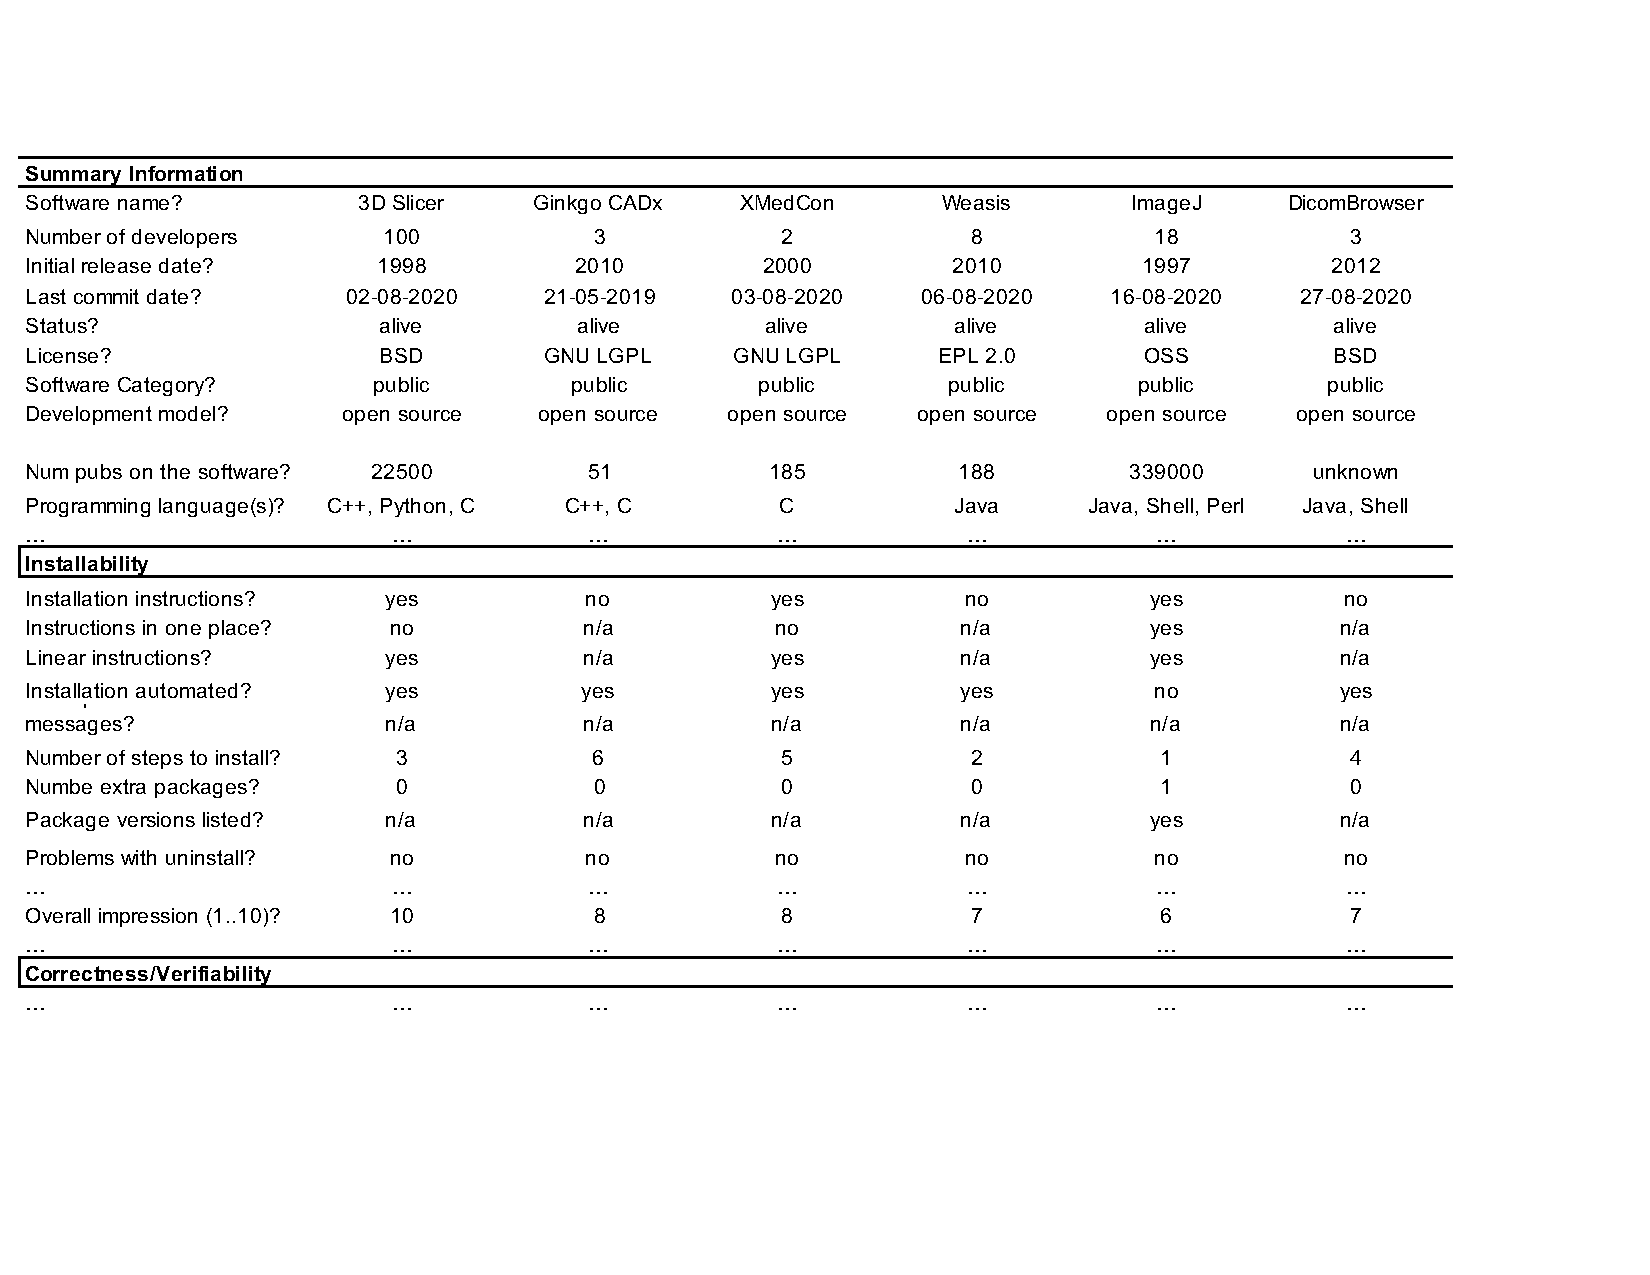
\includegraphics[scale=0.67]{template.pdf}
\caption{Grading template example}
\label{fg_grading_template_example}
\end{figure*}

The full template consists of 108 questions over 9 qualities.  These
questions are designed to be unambiguous, quantifiable, and measurable
with constrained time and domain knowledge.

The grader, after answering questions for each quality assigns an overall
score (between 1 and 10) based on the answers.  Several of the qualities use
the word ``surface'' to highlight that these particular qualities are a shallow
measure.  For example, usability is not measured using user studies.
Instead, we look for signs that the developers considered usability.
We use two freeware tools to collect repository related data:
\href{https://github.com/tomgi/git_stats}{GitStats} and
\href{https://github.com/boyter/scc}{Sloc Cloc and Code (scc)}.  Further
details on quality measurement are provided in [redacted for double blind].
%% DOUBLE BLIND
%Smith et al.\ (2024) \cite{SmithEtAl2024_MI_SOP}.

\subsubsection{Analytic Hierarchy Process (AHP)} \label{sec_AHP}

Developed by Saaty in the 1970s, AHP is widely used to analyze multiple criteria
decisions~\cite{VaidyaEtAl2006}. AHP organizes multiple criteria in a
hierarchical structure and uses pairwise comparisons between alternatives to
calculate relative ratios~\cite{Saaty1990}. AHP works with sets of $n$
\textit{options} and $m$ \textit{criteria}.  In our project $n=29$ and $m=9$
since there are 29 options (software products) and 9 criteria (qualities). With
AHP the sum of the grades (scores) for all products for a given quality will be
1.0.  We rank the software for each of the qualities, and then we combine the
quality rankings into an overall ranking based on the relative priorities
between qualities.

\subsubsection{Interview Methods} \label{sec_interview_methods}

The repository-based measurements are incomplete because they don't generally
capture the development process, the developer pain points, the perceived
threats to software quality, and the developers' strategies to address these
threats.  Therefore, part of our methodology involves interviewing developers.
We based our interviews on a list of 20 questions, which can be found in
[citation redacted for double blind].
%Smith et al. \cite{SmithEtAl2021}. 
Some questions are about the background of the software, the development teams,
the interviewees, and how they organize their projects.  We also ask about the
developer's understanding of the users. Some questions focus on the current and
past difficulties, and the solutions the team has found, or plan to try. We also
discuss documentation, both with respect to how it is currently done, and how it
is perceived. A few questions are about specific software qualities, such as
maintainability, understandability, usability, and reproducibility. The
interviews are semi-structured based on the question list.

\section{In-Scope Open-Source MI Software} \label{SecWhatProjects}

We initially identified 48 candidate software projects from the literature
\cite{Bjorn2017, Bruhschwein2019, Haak2015}, on-line articles \cite{Emms2019,
Hasan2020, Mu2019}, and forum discussions \cite{Samala2014}.  Then we filtered
as follows:

\begin{enumerate}

\item Removed the packages with no source code available, such as
\textit{MicroDicom}, \textit{Aliza}, and \textit{jivex}.

\item Focused on MI software that provides visualization functions.  We removed
seven packages that were toolkits or libraries, such as \textit{VTK},
\textit{ITK}, and \textit{dcm4che}, and another three that were for PACS.

\item Removed \textit{Open Dicom Viewer} as it has not received any
updates since 2011.

\end{enumerate}

The Domain Expert provided a list 12 software packages.  We found 6 packages
were on both lists: \textit{3D Slicer}, \textit{Horos}, \textit{ImageJ},
\textit{Fiji}, \textit{MRIcron} (we use its descendant \textit{MRIcroGL}) and
\textit{Mango} (we use the web version \textit{Papaya}).  The remaining six
packages were on our out-of-scope list. The Domain Expert agreed with our final
choice of 29 packages.  Table~\ref{tab_final_list} summarizes the in-scope
open-source MI software that is available at the time of measurement (the year
2020), thus answering \rqref{RQ_WhatProjects}.

\begin{table*}[!ht]
\centering
\begin{tabular}{p{3.7cm}lllllllll}
\toprule
\multirow{2}{*}{Software} & \multirow{2}{*}{Rlsd} & \multirow{2}{*}{Updated} & \multirow{2}{*}{Fnd} & \multirow{2}{*}{NOC} & \multirow{2}{*}{LOC} & \multicolumn{3}{c}{OS} & \multirow{2}{*}{Web} \\ \cmidrule{7-9}
 &  &  &  &  &  & W & M & L &  \\ \midrule
ParaView \cite{Ahrens2005} & 2002 & 2020-10 & \checkmark & 100 & 886326 & \checkmark & \checkmark & \checkmark & \checkmark \\
Gwyddion \cite{Nevcas2012} & 2004 & 2020-11 &  & 38 & 643427 & \checkmark & \checkmark & \checkmark &  \\
Horos \cite{horosproject2020} & ? & 2020-04 &  & 21 & 561617 &  & \checkmark &  &  \\
OsiriX Lite \cite{PixmeoSARL2019} & 2004 & 2019-11 &  & 9 & 544304 &  & \checkmark &  &  \\
3D Slicer \cite{Kikinis2014} & 1998 & 2020-08 & \checkmark & 100 & 501451 & \checkmark & \checkmark & \checkmark &  \\
Drishti \cite{Limaye2012} & 2012 & 2020-08 &  & 1 & 268168 & \checkmark & \checkmark & \checkmark &  \\
Ginkgo CADx \cite{Wollny2020} & 2010 & 2019-05 &  & 3 & 257144 & \checkmark & \checkmark & \checkmark &  \\
GATE \cite{Jan2004} & 2011 & 2020-10 &  & 45 & 207122 &  & \checkmark & \checkmark &  \\
3DimViewer \cite{TESCAN2020} & ? & 2020-03 & \checkmark & 3 & 178065 & \checkmark & \checkmark &  &  \\
medInria \cite{Fillard2012} & 2009 & 2020-11 &  & 21 & 148924 & \checkmark & \checkmark & \checkmark &  \\
BioImage Suite Web \cite{Papademetris2005} & 2018 & 2020-10 & \checkmark & 13 & 139699 &
\checkmark & \checkmark & \checkmark & \checkmark \\
Weasis \cite{Roduit2021} & 2010 & 2020-08 &  & 8 & 123272 & \checkmark & \checkmark & \checkmark &  \\
AMIDE \cite{Loening2017} & 2006 & 2017-01 &  & 4 & 102827 & \checkmark & \checkmark & \checkmark &  \\
XMedCon \cite{Nolf2003} & 2000 & 2020-08 &  & 2 & 96767 & \checkmark & \checkmark & \checkmark &  \\
ITK-SNAP \cite{Yushkevich2006} & 2006 & 2020-06 & \checkmark & 13 & 88530 & \checkmark & \checkmark & \checkmark &  \\
Papaya \cite{UTHSCSA2019} & 2012 & 2019-05 &  & 9 & 71831 & \checkmark & \checkmark & \checkmark &  \\
OHIF Viewer \cite{Ziegler2020} & 2015 & 2020-10 &  & 76 & 63951 & \checkmark & \checkmark & \checkmark & \checkmark \\
SMILI \cite{Chandra2018} & 2014 & 2020-06 &  & 9 & 62626 & \checkmark & \checkmark & \checkmark &  \\
INVESALIUS 3 \cite{Amorim2015} & 2009 & 2020-09 &  & 10 & 48605 & \checkmark & \checkmark & \checkmark &  \\
dwv \cite{Martelli2021} & 2012 & 2020-09 &  & 22 & 47815 & \checkmark & \checkmark & \checkmark & \checkmark \\
DICOM Viewer \cite{Afsar2021} & 2018 & 2020-04 & \checkmark & 5 & 30761 & \checkmark & \checkmark & \checkmark &  \\
MicroView \cite{ParallaxInnovations2020} & 2015 & 2020-08 &  & 2 & 27470 & \checkmark & \checkmark & \checkmark &  \\
MatrixUser \cite{Liu2016} & 2013 & 2018-07 &  & 1 & 23121 & \checkmark & \checkmark & \checkmark &  \\
Slice:Drop \cite{Haehn2013} & 2012 & 2020-04 &  & 3 & 19020 & \checkmark & \checkmark & \checkmark & \checkmark \\
dicompyler \cite{Panchal2010} & 2009 & 2020-01 &  & 2 & 15941 & \checkmark & \checkmark &  &  \\
Fiji \cite{Schindelin2012} & 2011 & 2020-08 & \checkmark & 55 & 10833 & \checkmark & \checkmark & \checkmark &  \\
ImageJ \cite{Rueden2017} & 1997 & 2020-08 & \checkmark & 18 & 9681 & \checkmark & \checkmark & \checkmark &  \\
MRIcroGL \cite{Rorden2021} & 2015 & 2020-08 &  & 2 & 8493 & \checkmark & \checkmark & \checkmark &  \\
DicomBrowser \cite{Archie2012} & 2012 & 2020-08 &  & 3 & 5505 & \checkmark & \checkmark & \checkmark &  \\ \bottomrule
\end{tabular}
\caption{Final software list (sorted in descending order of the number of Lines
Of Code (LOC))}
\label{tab_final_list}
\end{table*}

In Table~\ref{tab_final_list} the projects are sorted in descending order of
lines of code.  We found the initial release dates (Rlsd) for most projects and
marked the two unknown dates with ``?''. The date of the last update is the date
of the latest update, at the time of measurement. We found funding information
(Fnd) for only eight projects.  For the Number Of Contributors (NOC) we
considered anyone who made at least one accepted commit as a contributor. The
NOC is not usually the same as the number of long-term project members, since
many projects received change requests and code from the community.  With
respect to the OS, 25 packages work on all three OSs: Windows (W), macOS (M),
and Linux (L). Although the usual approach to cross-platform compatibility was
to work natively on multiple OSes, five projects achieved platform-independence
via web applications. The full measurement data for all packages is available on
[removed for blind review]
%\href{https://data.mendeley.com/datasets/k3pcdvdzj2/1} {Mendeley Data}.  
%% DOUBLE BLIND

The programming languages used in order of decreasing popularity are \CC,
JavaScript, Java, C, Python, Pascal, Matlab.  The most popular language is \CC,
for 11 of 29 projects; Pascal and Matlab were each used for a single project.

\section{Which Projects Follow Best Practices?} \label{SecMeasurementResults}

To answer \rqref{RQ_HighestQuality} we measured the software as described in
Section~\ref{SecMethodology}.  In the absence of a specific real world context,
we assumed all nine qualities are equally important.
Figure~\ref{fg_overall_scores} shows the overall AHP scores in descending order.

\begin{figure*}[!ht]
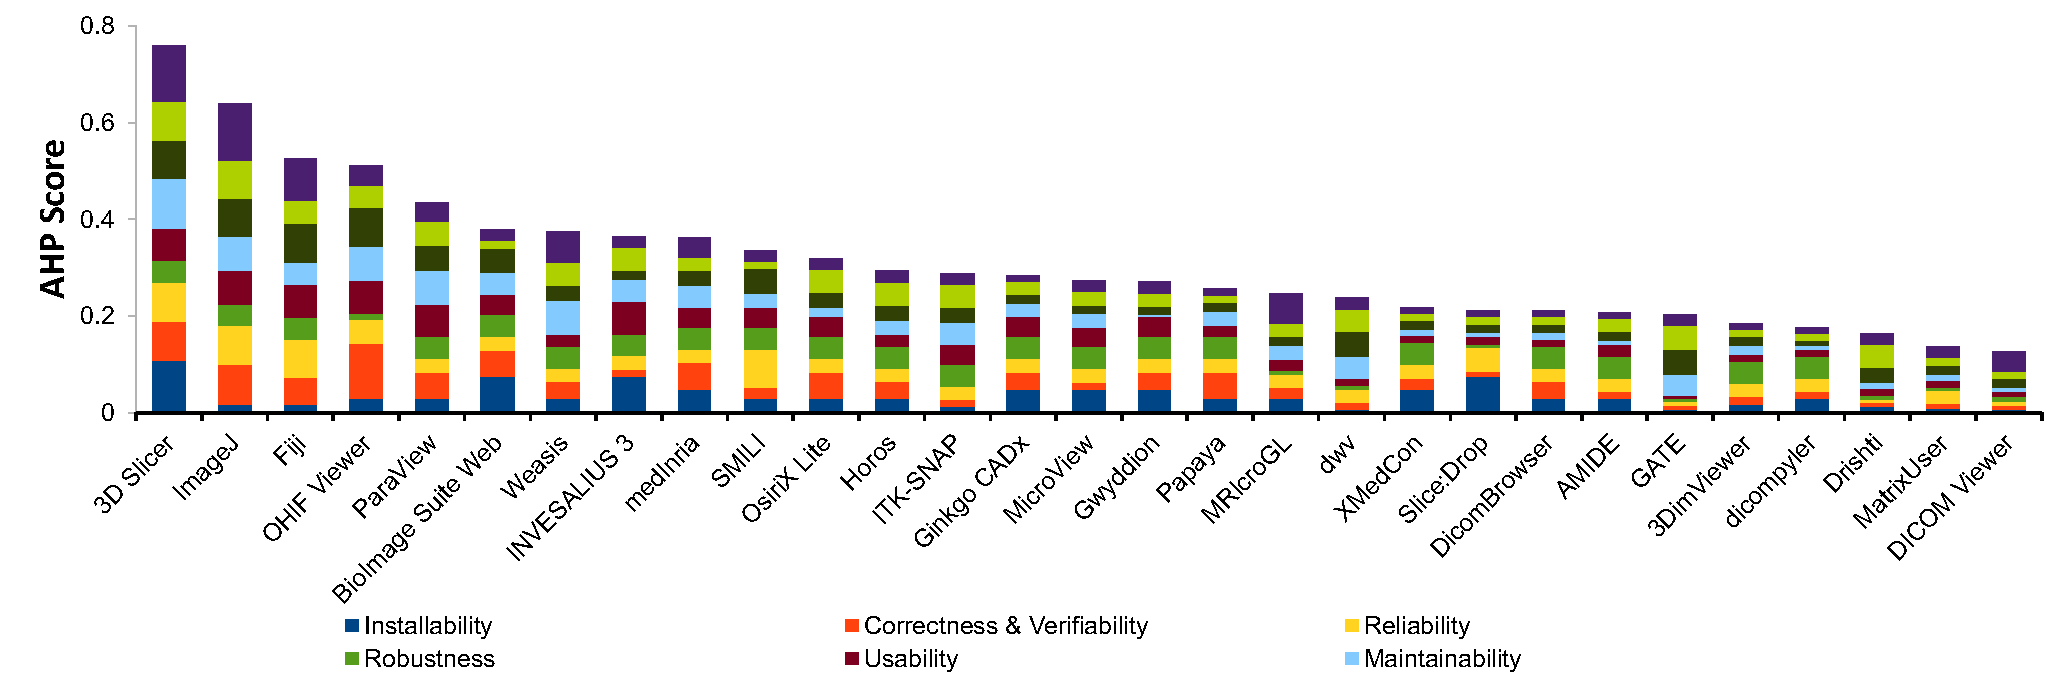
\includegraphics[scale=0.47]{overall_scores.pdf}
\caption{Overall AHP scores with an equal weighting for all 9 software qualities}

\label{fg_overall_scores}
\end{figure*}

The top four software products \textit{3D Slicer}, \textit{ImageJ},
\textit{Fiji}, and \textit{OHIF Viewer} have higher scores in most criteria.
\textit{3D Slicer} has a score in the top two for all qualities; \textit{ImageJ}
ranks near the top for all qualities, except for correctness \& verifiability.
\textit{OHIF Viewer} and \textit{Fiji} have similar overall scores, with
\textit{Fiji} doing better in installability and \textit{OHIF Viewer} doing
better in correctness \& verifiability.  Given the installation problems, we may
have underestimated the scores on reliability and robustness for \textit{DICOM
Viewer}, but we compared it equally for the other seven qualities.

The overall score is based on the measurement of the identified qualities. Full
details of how the projects compare for each quality can be found in [citation
redacted for blind review].
%% DOUBLE BLIND
%Smith et al.~\cite{SmithEtAl2024_MI_SOP}
The highlights are as follows:

\begin{description}

\item [Installability] We found installation instructions for 16 projects, but
two did not need them (\textit{BioImage Suite Web} and \textit{Slice:Drop}) as
they are web applications. 10 of the projects required extra dependencies: Five
depend on a specific browser; \textit{dwv}, \textit{OHIF Viewer}, and
\textit{GATE} needs extra libraries to build; \textit{ImageJ} and \textit{Fiji}
need an unzip tool; \textit{MatrixUser} needs Matlab; \textit{DICOM Viewer}
needs a Nextcloud platform. \textit{GATE}, \textit{dwv}, and \textit{DICOM
Viewer} showed severe installation problems. We were not able to install them,
even after a reasonable amount of time (2 hours).

\item [Correctness \& Verifiability] The packages with higher scores for
correctness and verifiability used a wider array of techniques to improve
correctness, and had better documentation to witness this.  For instance, we
looked for evidence of unit testing, and found evidence for only about half of
the projects. We identified five projects using continuous integration tools:
\textit{3D Slicer}, \textit{ImageJ}, \textit{Fiji}, \textit{dwv}, and
\textit{OHIF Viewer}. The only requirements-related document we found was a road
map of \textit{3D Slicer}, which contained design requirements for upcoming
changes.

\item [Surface Reliability] We were able to follow the steps in the tutorials
that existed (seven packages had them.) However, \textit{GATE} could not open
macro files and became unresponsive several times, without any descriptive error
message. We found that \textit{Drishti} crashed when loading damaged image
files, without showing any descriptive error message.

\item [Surface Robustness] According to their documentation, all 29 software
packages should support the DICOM standard. To test robustness, we prepared two
types of image files: correct and incorrect formats (with the incorrect format
created by relabelling a text file to have the ``.dcm'' extension).  All
software packages loaded the correct format image, except for \textit{GATE},
which failed for unknown reasons.  For the broken format, \textit{MatrixUser},
\textit{dwv}, and \textit{Slice:Drop} ignored the incorrect format, did not show
any error message and displayed a blank image.  \textit{MRIcroGL} behaved
similarly except that it showed a meaningless image.  \textit{Drishti}
successfully detected the broken format of the file, but the software crashed as
a result.

\item [Surface Usability] The software with higher usability scores usually
provided both comprehensive documented guidance and a good user experience.
\textit{INVESALIUS 3} provided an excellent example of a detailed and precise
user manual. \textit{GATE} also provided numerous documents, but unfortunately
we had difficulty understanding and using them. We found getting started
tutorials for only 11 projects, but a user manual for 22 projects.
\textit{MRIcroGL} was the only project that explicitly documented expected user
characteristics.

\item [Maintainability] We gave \textit{3D Slicer} the highest score for
maintainability because we found it had the most comprehensive artifacts. Only a
few of the 29 projects had a product, developer's manual, or API (Application
Programming Interface) documentation, and only \textit{3D Slicer},
\textit{ImageJ}, \textit{Fiji} included all three documents.  Moreover,
\textit{3D Slicer} has a much higher percentage of closed issues (92\%) compared
to \textit{ImageJ} (52\%) and \textit{Fiji} (64\%). Twenty-seven of the 29
projects used git for version control, with 24 of these using GitHub.
\textit{AMIDE} used Mercurial and \textit{Gwyddion} used Subversion.
\textit{XMedCon}, \textit{AMIDE}, and \textit{Gwyddion} used SourceForge.
\textit{DicomBrowser} and \textit{3DimViewer} used BitBucket. 

\item [Reusability] We have assumed that smaller code files are
likely more reusable -- see Table \ref{tab_loc_per_file} for the details.

\item [Surface Understandability] All projects had a consistent coding style
with parameters in the same order for all functions, modularized code, and,
clear comments that indicate what is done, not how. However, we only found
explicit identification of a coding standard for 3 out of the 29: \textit{3D
Slicer}, \textit{Weasis}, and \textit{ImageJ}. We also found hard-coded
constants (rather than symbolic constants) in \textit{medInria},
\textit{dicompyler}, \textit{MicroView}, and \textit{Papaya}. We did not find
any reference to the algorithms used in projects \textit{XMedCon},
\textit{DicomBrowser}, \textit{3DimViewer}, \textit{BioImage Suite Web},
\textit{Slice:Drop}, \textit{MatrixUser}, \textit{DICOM Viewer},
\textit{dicompyler}, and \textit{Papaya}. 

\item [Visibility/Transparency] Generally speaking, the teams that actively
documented their development process and plans scored higher.  \textit{3D
Slicer} and \textit{ImageJ} were the only projects to include documentation for
all of the following: development process, project status, development
environment and release notes.

\end{description}  

\begin{table*}[!ht]
\centering
\begin{tabular}{lllll}
\toprule
\multirow{2}{*}{Software} & \multirow{2}{*}{Text Files} & \multirow{2}{*}{Total Lines} & \multirow{2}{*}{LOC} & \multirow{2}{*}{LOC/file} \\
 &  &  &  &  \\ 
\midrule
OHIF Viewer & 1162 & 86306 & 63951 & 55 \\
3D Slicer & 3386 & 709143 & 501451 & 148 \\
Gwyddion & 2060 & 787966 & 643427 & 312 \\
ParaView & 5556 & 1276863 & 886326 & 160 \\
OsiriX Lite & 2270 & 873025 & 544304 & 240 \\
Horos & 2346 & 912496 & 561617 & 239 \\
medInria & 1678 & 214607 & 148924 & 89 \\
Weasis & 1027 & 156551 & 123272 & 120 \\
BioImage Suite Web & 931 & 203810 & 139699 & 150 \\
GATE & 1720 & 311703 & 207122 & 120 \\
Ginkgo CADx & 974 & 361207 & 257144 & 264 \\
SMILI & 275 & 90146 & 62626 & 228 \\
Fiji & 136 & 13764 & 10833 & 80 \\
Drishti & 757 & 345225 & 268168 & 354 \\
ITK-SNAP & 677 & 139880 & 88530 & 131 \\
3DimViewer & 730 & 240627 & 178065 & 244 \\
DICOM Viewer & 302 & 34701 & 30761 & 102 \\
ImageJ & 40 & 10740 & 9681 & 242 \\
dwv & 188 & 71099 & 47815 & 254 \\
MatrixUser & 216 & 31336 & 23121 & 107 \\
INVESALIUS 3 & 156 & 59328 & 48605 & 312 \\
AMIDE & 183 & 139658 & 102827 & 562 \\
Papaya & 110 & 95594 & 71831 & 653 \\
MicroView & 137 & 36173 & 27470 & 201 \\
XMedCon & 202 & 129991 & 96767 & 479 \\
MRIcroGL & 97 & 50445 & 8493 & 88 \\
Slice:Drop & 77 & 25720 & 19020 & 247 \\
DicomBrowser & 54 & 7375 & 5505 & 102 \\
dicompyler & 48 & 19201 & 15941 & 332 \\ 
\bottomrule
\end{tabular}
\caption{Number of files and lines (by reusability scores)}
\label{tab_loc_per_file}
\end{table*}

\section{Comparison to Community Ranking} \label{Sec_VsCommunityRanking}

To answer \rqref{RQ_CompareHQ2Popular} we use GitHub stars, number of forks and
number of people watching the projects are proxies for community ranking.
Table~\ref{tab_ranking_vs_GitHub} show the statistics for data collected in July
2021.  Recall that 24 projects use GitHub (Section~\ref{SecMeasurementResults}).

Our ranking and GitHub popularity, at least for the top five projects, seems to
line up fairly well. However, we ranked some popular packages fairly low, such
as \textit{dwv}. This is because we were unable to build it locally, even though
we followed its installation instructions. However, we were able to use its web
version for the rest of the measurements. Additionally, this version did not
detect a broken DICOM file and instead displayed a blank image
(Section~\ref{SecMeasurementResults}).  \textit{DICOM Viewer} ranked low as we
were unable to install the NextCloud platform.

Another likely reason for discrepancies is that we weighted all qualities
equally. This is not likely how users implicitly rank the different qualities.
This would require a broader user study to properly assess. Furthermore our
measures of popularity are only \emph{proxies} which are biased towards
past rather than current preferences~\cite{Szulik2017}, as these are
monotonically increasing quantities. Finally there are often more factors than
just quality that influence the popularity of ``consumer'' products.

\begingroup
\renewcommand{\arraystretch}{0.85}
\begin{table*}[!ht]
\centering
\begin{tabular}{llllll}
\toprule
Software & Comm.\ Rank & Our Rank & Stars/yr & Watches/yr & Forks/yr \\ 
\midrule
3D Slicer & 1 & 1 & 284 & 19 & 128 \\
OHIF Viewer & 2 & 4 & 277 & 19 & 224 \\
dwv & 3 & 19 & 124 & 12 & 51 \\
ImageJ & 4 & 2 & 84 & 9 & 30 \\
ParaView & 5 & 5 & 67 & 7 & 28 \\
Horos & 6 & 12 & 49 & 9 & 18 \\
Papaya & 7 & 17 & 45 & 5 & 20 \\
Fiji & 8 & 3 & 44 & 5 & 21 \\
DICOM Viewer & 9 & 29 & 43 & 6 & 9 \\
INVESALIUS 3 & 10 & 8 & 40 & 4 & 17 \\
Weasis & 11 & 7 & 36 & 5 & 19 \\
dicompyler & 12 & 26 & 35 & 5 & 14 \\
OsiriX Lite & 13 & 11 & 34 & 9 & 24 \\
MRIcroGL & 14 & 18 & 24 & 3 & 3 \\
GATE & 15 & 24 & 19 & 6 & 26 \\
Ginkgo CADx & 16 & 14 & 19 & 4 & 6 \\
BioImage Suite Web & 17 & 6 & 18 & 5 & 7 \\
Drishti & 18 & 27 & 16 & 4 & 4 \\
Slice:Drop & 19 & 21 & 10 & 2 & 5 \\
ITK-SNAP & 20 & 13 & 9 & 1 & 4 \\
medInria & 21 & 9 & 7 & 3 & 6 \\
SMILI & 22 & 10 & 3 & 1 & 2 \\
MatrixUser & 23 & 28 & 2 & 0 & 0 \\
MicroView & 24 & 15 & 1 & 1 & 1 \\
Gwyddion & 25 & 16 & n/a & n/a & n/a \\
XMedCon & 26 & 20 & n/a & n/a & n/a \\
DicomBrowser & 27 & 22 & n/a & n/a & n/a \\
AMIDE & 28 & 23 & n/a & n/a & n/a \\
3DimViewer & 29 & 25 & n/a & n/a & n/a \\ 
\bottomrule
\end{tabular}
\caption{Software ranking by our methodology versus the community (Comm.)\
ranking using GitHub metrics (Sorted in descending order of community
popularity, as estimated by the number of new stars per year)}
\label{tab_ranking_vs_GitHub}
\end{table*}
\endgroup

Although both rankings are imperfect measures, they nevertheless suggest a
correlation between best practices and popularity. We don't know if this is
causal, in either direction (i.e. if best practices enable popularity or if
popularity increases the need for using more software development best
practices).

\section{Compare to Recommended Software Artifacts} \label{Sec_CompareArtifacts}

For \rqref{RQ_CompareArtifacts} we use nine research software development
guidelines to compare recommended software artifacts versus those present in MI
software.  These guidelines are:
\begin{itemize}
\item United States Geological Survey Software Planning Checklist
\cite{USGS2019},
\item DLR (German Aerospace Centre) Software Engineering Guidelines
\cite{TobiasEtAl2018}, 
\item Scottish Covid-19 Response Consortium Software Checklist
\cite{BrettEtAl2021},
\item Good Enough Practices in Scientific Computing \cite{WilsonEtAl2016},
\item xSDK (Extreme-scale Scientific Software Development Kit) Community Package
Policies \cite{SmithAndRoscoe2018},
\item Trilinos Developers Guide \cite{HerouxEtAl2008},
\item EURISE (European Research Infrastructure Software Engineers') Network
Technical Reference \cite{ThielEtAl2020},
\item CLARIAH (Common Lab Research Infrastructure for the Arts and Humanities)
Guidelines for Software Quality \cite{vanGompelEtAl2016}, and
\item A Set of Common Software Quality Assurance Baseline Criteria for Research
Projects \cite{OrvizEtAl2017}.
\end{itemize}

\begin{table*}[!ht]
\begin{center}
\begin{tabular}{ p{3.5cm}p{0.5cm}p{0.5cm}p{0.5cm}p{0.5cm}p{0.5cm}p{0.5cm}p{0.5cm}p{0.5cm}p{0.5cm}p{0.5cm} }
\toprule
~ \ & \cite{USGS2019} & \cite{TobiasEtAl2018} & \cite{BrettEtAl2021} &
\cite{WilsonEtAl2016} & \cite{SmithAndRoscoe2018} & \cite{HerouxEtAl2008} &
\cite{ThielEtAl2020} & \cite{vanGompelEtAl2016} & \cite{OrvizEtAl2017} & MI\\
\midrule
LICENSE & \checkmark & \checkmark & \checkmark & \checkmark & \checkmark & &
\checkmark & \checkmark & \checkmark & C\\
README &  & \checkmark & \checkmark & \checkmark & \checkmark & & \checkmark &
\checkmark & \checkmark & C\\
CONTRIBUTING &  & \checkmark & \checkmark & \checkmark & \checkmark & &
\checkmark & \checkmark & \checkmark & R\\
CITATION &  &  &  & \checkmark & & & & \checkmark & \checkmark & U\\
CHANGELOG &  & \checkmark &  & \checkmark & \checkmark & & \checkmark &  &  & U\\
INSTALL &  &  &  &  & \checkmark & & \checkmark & \checkmark & \checkmark & U\\
\midrule
Uninstall &  &  &  &  & & & & \checkmark & &  \\
Dependency List &  &  & \checkmark & & \checkmark & & & \checkmark &  & R\\
Authors &  &  &  &  &  &  & \checkmark & \checkmark & \checkmark & U\\
Code of Conduct &  &  &  &  & & & \checkmark & & & R\\
Acknowledgements &  &  &  &  &  &  & \checkmark & \checkmark & \checkmark & U\\
Code Style Guide &  & \checkmark &  &  & & & \checkmark & \checkmark & \checkmark & R\\
Release Info. &  & \checkmark &  &  & & \checkmark & \checkmark & & & C\\
Prod.\ Roadmap &  &  &  &  & & \checkmark & \checkmark & \checkmark & & R\\
\midrule
Getting started &  &  &  &  & \checkmark & & \checkmark & \checkmark & \checkmark & R\\
User manual &  &  & \checkmark &  & & & \checkmark & & & C\\
Tutorials &  &  &  &  & & & \checkmark & & & U\\
FAQ &  &  &  &  & & & \checkmark & \checkmark & \checkmark & U\\
\midrule
Issue Track &  & \checkmark & \checkmark & & \checkmark & \checkmark &
\checkmark & & \checkmark & C\\
Version Control &  & \checkmark & \checkmark & \checkmark & \checkmark &
\checkmark & \checkmark & \checkmark & \checkmark & C\\ 
Build Scripts &  & \checkmark &  & \checkmark & \checkmark & \checkmark &
\checkmark & & \checkmark & U\\
\midrule
Requirements &  & \checkmark &  &  & & \checkmark &  &  & \checkmark & R\\
Design Doc.\ &  & \checkmark  & \checkmark &  & \checkmark & & \checkmark &
\checkmark& \checkmark & R\\
API Doc. &  &  &  &  & \checkmark & & \checkmark & \checkmark & \checkmark & R\\
Test Plan &  & \checkmark &  &  & & \checkmark & & & &  \\
Test Cases & \checkmark & \checkmark & \checkmark &  & \checkmark & \checkmark &
\checkmark & \checkmark & \checkmark & U\\
\bottomrule
\end{tabular}
\caption{Comparison of Recommended Artifacts in Software Development Guidelines
to Artifacts in MI Projects (C for Common, U for Uncommon and R for Rare)}
\label{Tbl_Guidelines}
\end{center}
\end{table*}

In Table~\ref{Tbl_Guidelines} each row corresponds to an artifact.  For a given
row, a checkmark in one of the columns means that the corresponding guideline
recommends this artifact.  The last column shows whether the artifact appears in
the measured set of MI software, either not at all (blank), commonly (C),
uncommonly (U) or rarely (R).  We did our best to interpret the meaning of each
artifact consistently between guidelines and specific MI software, but the
terminology and the contents of artifacts are not standardized.  The challenge
even exists for the ubiquitous README file.  The content of README files shows
significant variation between projects \cite{PranaEtAl2018}.  Although some
content is reasonably consistent, with 97\% of README files contain at least one
section describing the `What' of the repository and 89\% offering some `How'
content, other categories are more variable.  For instance, information on
`Contribution', `Why', and `Who', appear in 28\%, 26\% and 53\% of the analyzed
files, respectively \cite{PranaEtAl2018}.  

\begin{table*}[!ht]
    \begin{center}
    \begin{tabular}{ p{3.8 cm} p{6.4 cm} p{4.5 cm}}
    \toprule
    Common & Uncommon & Rare \\
    \midrule
    README (29) & Build scripts (18) & Getting Started (9)\\
    Version control (29) & Tutorials (18) & Developer's manual (8)\\
    License (28) & Installation guide (16) & Contributing (8)\\
    Issue tracker (28) & Test cases (15) & API documentation (7)\\
    User manual (22) & Authors (14) & Dependency list (7)\\
    Release info. (22) & Frequently Asked Questions (14) & Troubleshooting guide (6)\\
     & Acknowledgements (12) & Product roadmap (5)\\
     & Changelog (12) & Design documentation (5)\\
     & Citation (11) & Code style guide (3)\\
     & & Code of conduct (1)\\
     & & Requirements (1)\\
    \bottomrule
    \end{tabular}
    \caption{Artifacts Present in MI Packages, Classified by Frequency (The number 
    in brackets is the number of occurrences)}
    \label{artifactspresent}
    \end{center}
\end{table*}

Table~\ref{artifactspresent} presents our measurements for MI software.
The table groups the artifacts by frequency
into categories of common (20 to 29 ($>$67\%) packages), uncommon (10 to 19
(33-67\%) packages), and rare (1 to 9 ($<$33\%) packages).

Note that ``popularity'' in Table~\ref{Tbl_Guidelines} does no imply that these
oft recommended artifacts are the most important. Guidelines are often brief,
to encourage adoption, and thus even guidelines that mention the need for
installation instructions rarely mention uninstallation instructions.
Two items in Table~\ref{artifactspresent} do not appear in any guidelines:
\emph{Troubleshooting guide} and \emph{Developer's manual}.  However the
information within these documents overlaps with
the recommended artifacts.  Troubleshooting information often can be found in
a User Manual, while the information in a ``Developer's Manual'' is often
scattered amongst many other documents.

Three of the 26 recommended artifacts were never observed in the MI software:
i) Uninstall, ii) Test plans, and iii) Requirements. It is possible that
some of these were created but never put under version control.

Neglecting requirements documentation is unfortunately common for research
software, and MI software is no exception to this trend.  Although such
documentation is recommended by some \cite{TobiasEtAl2018, HerouxEtAl2008,
SmithAndKoothoor2016}, in practice this is rare~\cite{HeatonAndCarver2015}.
Sanders and Kelly \cite{SandersAndKelly2008} interviewed 16 scientists from 10
disciplines and found that none of the scientists created requirements
specifications, unless regulations in their field mandated such a document.
Requirements are the least commonly produced type of documentation for research
software in general \cite{Nguyen-HoanEtAl2010}. 

This is unfortunate as when scientific developers are surveyed on their pain
points, Wiese et al.~\cite{WieseEtAl2019} found that software requirements and
management is the software engineering discipline that most hurts them,
accounting for 23\% of the technical problems reported by study participants.
Further adding to the misfortune, there is a widespread perception that up-front
requirements are impossible for research software \cite{CarverEtAl2007,
SegalAndMorris2008}. Fortunately a more agile approach to requirements is
feasible~\cite{Smith2016}, and research-software specific templates
exist~\cite{SmithEtAl2007}. 

A theme emerges amongst the artifacts rarely observed in practice: they
are developer-focused (a list of library dependencies, a contributor's guide,
a developer Code of Conduct, coding style guidelines, product roadmap, design
documentation and API documentation).

Other communities use checklists to help with best practices. Examples include
checklists for merging branches~\cite{Brown2015}, for saving and sharing changes
to the project~\cite{WilsonEtAl2016}, for new and departing team
members~\cite{HerouxAndBernholdt2018}, for processes related to commits and
releases~\cite{HerouxEtAl2008} and for overall software
quality~\cite{ThielEtAl2020, SSI2022}.

MI projects fall somewhat short of recommended best practices, but are not alone
amongst research software projects. This gap has been documented
before~\cite{Storer2017,JohansonAndHasselbring2018}, and is known to cause
sustainability and reliability problems \cite{FaulkEtAl2009}, and to waste
development effort~\cite{deSouzaEtAl2019}.

\section{Comparison of Tool Usage Between MI and Other Research Software}
\label{Sec_CompareTools}

We use data from interviews, as described in Section~\ref{sec_interview_methods}
to answer \rqref{RQ_CompareToolsProjMngmnt}, \rqref{RQ_CompareMethodologies}
and \rqref{RQ_PainPoints}. Requests were sent to all 29 projects.  Nine
developers from eight of the projects agreed to participate: \textit{3D Slicer},
\textit{INVESALIUS 3}, \textit{dwv}, \textit{BioImage Suite Web},
\textit{ITK-SNAP}, \textit{MRIcroGL}, \textit{Weasis}, and \textit{OHIF}. We
spent about 90 minutes for each interview. The full interview answers can be
found in [citation redacted for blind review].
%\cite{Dong2021}.

Developers use software tools for user support, version control, Continuous
Integration and Deployment (CI/CD), documentation and project management. To
answer \rqref{RQ_CompareToolsProjMngmnt}, we summarize the tool usage in these
categories, and compare this to the usage by the research software community.

Table~\ref{tab_user_support_model} summarizes the user support models by the
number of projects using each model (projects may use more than one support
model). The prevalent usage of GitHub issues may be by design, or it might just
naturally arise as users seek help.

\begin{table}[!ht]
\centering
\begin{tabular}{lc}
\toprule
\multicolumn{1}{c}{User Support Model} & Num.\ Projects \\
\midrule
GitHub issue & 24 \\
Frequently Asked Questions (FAQ) & 12 \\
Forum & 10 \\
E-mail address & 9 \\
GitLab issue, SourceForge discussions & 2 \\
Troubleshooting & 2 \\
Contact form & 1 \\ 
\bottomrule
\end{tabular}
\caption{\label{tab_user_support_model}User support models by number of projects}
\end{table}

Most teams interview (eight of nine) mentioned using GitHub and pull requests to manage
contributions from the community. The interviewees generally gave very positive
feedback on using GitHub. Some teams previously used a different approach to
version control and eventually transferred to git and GitHub.

The common use of version control for MI software illustrates considerable
improvement from the poor adoption of version control tools that Wilson lamented
in 2006 \cite{Wilson2006}.  The proliferation of version control tools for MI
matches the increase in the broader research software community.  A little over
10 years ago Nguyen-Hoan et al.\ \cite{Nguyen-HoanEtAl2010} estimated that only
50\% of research software projects used version control, but even at that time
there was an increase from previous usage levels. A survey in 2018 shows 81\% of
developers use a version control system \cite{AlNoamanyAndBorghi2018}.
\cite{Smith2018} has similar results, showing version control usage for alive
projects in mesh generation, geographic information systems and statistical
software for psychiatry increasing from 75\%, 89\% and 17\% (respectively) to
100\%, 95\% and 100\% (respectively) over a four-year period ending in 2018. A
recent survey by \cite{CarverEtAl2022} shows version control use among
practitioners at over 95\%. All but one of the software guides cited in
Section~\ref{Sec_CompareArtifacts} recommends version control. The high usage of
version control tools in MI matches the general trend in research software.

As mentioned in Section~\ref{SecMeasurementResults}, we identified 17\% of MI
projects using CI/CD tools. We found which projects used CI/CD by examining the
documentation and source code. The count of CI/CD usage may be higher, since
traces of CI/CD may not always appear in a repository.  This was the case for a
study of Lattice Boltzmann Method (LBM) software, where interviews with
developers showed that more projects used CI/CD than was evident from repository
artifacts alone [citation redacted for blind review].  %\cite{Michalski2021}.  
The 17\% utilization for MI software contrasts with the high frequency with
which research software development guidelines recommend continuous integration
\cite{BrettEtAl2021, Brown2015, ThielEtAl2020, Zadka2018, vanGompelEtAl2016}.
Although there is currently little data available on CI/CD utilization for
research software, our impression is that CI/CD is not yet common practice,
despite its recommendation.  This is certainly the case for LBM software, where
usage numbers sit around 12.5\% [citation redacted for blind review]
%\cite{Michalski2021}.  
The survey of \cite{CarverEtAl2022} suggests higher use of CI/CD with 54\%
(54/100) of respondents indicating that they use it. However, that study surveys
practitioners, rather than assessing projects.  Additional information on CI/CD
is given in the recommendations (Section~\ref{Sec_ContinuousIntegration}).

For documentation tools and methods mentioned by the interviewees, the most
popular (mentioned by about 30\% of developers) were forum discussions and
videos.  The second most popular options (mentioned by about 20\% of developers)
were GitHub, wiki pages, workshops, and social media. The least frequently
mentioned options (about 10\% of developers) included writing books, and google
forms.  In contrasting MI software with LBM software, the most significant
documentation tool difference is that LBM software often uses document
generation tools, like doxygen and sphinx [citation redacted for blind review].
%\cite{Michalski2021}

The interviewees talked about two types of project management tools:
\begin{inparaenum}[i)]
\item trackers, including GitHub, issue trackers, bug trackers and Jira; and,
\item documentation tools, including GitHub, Wiki page, Google Doc, and
Confluence.
\end{inparaenum}
Of the specifically named tools, interviewees mentioned GitHub 3 times, and each
of the other tools once each.

Based on information provided by \cite{JungEtAl2022}, tool utilization for MI
software has much in common with tool utilization for ocean modelling software.
Both use tools for editing, compiling, code management, testing, building, and
project management.  From the data available, ocean modelling differs from MI
software in its use of Kanban boards for project management.

\section[Comparison to Other Research Software]{Comparison of Principles, Process, and
Methodologies to Research Software in General} \label{Sec_CompareMethodologies}

We answer research question \rqref{RQ_CompareMethodologies} by comparing the
principles, processes, and methodologies used for MI software to what can be
gleaned from the literature on research software in general. In our interviews
with developers the responses about development model were vague, with only two
interviewees following a definite development model. In some cases the
interviewees felt their process was similar to an existing development model.
Three teams (about 38\%) either followed agile, or something similar to agile.
Two teams (25\%) either followed a waterfall process, or something similar.
Three teams (about 38\%) explicitly stated that their process was undefined or
self-directed.

Our observations of an informally defined process, with elements of agile
methods, matches observations for research software in general.
Scientific developers naturally use an agile philosophy \cite{AckroydEtAl2008,
CarverEtAl2007, EasterbrookAndJohns2009, Segal2005, HeatonAndCarver2015}, or an
amethododical process \cite{Kelly2013}, or a knowledge acquisition driven
process \cite{Kelly2015}.  A waterfall-like process can work for research
software \cite{Smith2016}, especially if the developers work iteratively and
incrementally, but externally document their work as if they followed a
rationale design process \cite{parnas1986rational}.

No interviewee introduced any strictly defined project management process. The
most common approach was following the issues, such as bugs and feature
requests. The \textit{3D Slicer} team had weekly meetings to
discuss the goals for the project. The \textit{INVESALIUS 3} team relied on the
GitHub process for their project management while the \textit{ITK-SNAP} team had a
fixed six-month release pace. Only the interviewee from \textit{OHIF} 
mentioned the team having a project manager. The \textit{3D Slicer} team and
\textit{BioImage Suite Web} team do nightly builds and tests. The \textit{OHIF}
developer believes that a better project management process can improve junior
developer efficiency while also improving internal and external communication.

We identified the use of unit testing in less than half of the 29 projects even
though the interviewees believed that testing (including usability tests with
users) was the top approach to improve correctness, usability, and
reproducibility.  This level of testing matches what was observed for LBM
software [citation redacted for blind review]
%\cite{Michalski2021} 
and is apparently greater than the level of
testing for ocean modelling software \cite{JungEtAl2022}.

Interviewees from all of the eight projects thought that documentation was
essential to their projects, and most of them (7 of 8) said that it could save
their time to answer questions from users and developers. Half of them (4 of 8)
saw the need to improve their documentation, and only three of them thought that
their documentations conveyed information clearly enough.

As Table~\ref{Tbl_Guidelines} suggests, an emphasis on documentation, especially
for new developers, is echoed in research software guidelines. Multiple
guidelines recommend a document explaining how to contribute to a project, often
named CONTRIBUTING. Guidelines also recommend tutorials, user guides and quick
start examples. \cite{SmithAndRoscoe2018} suggests including instructions
specifically for on-boarding new developers. For open-source software in general
(not just research software), \cite{Fogel2005} recommends providing tutorial
style examples, developer guidelines, demos, and screenshots.

\section{Developer Pain Points} \label{painpoints}

Based on interviews with nine developers (described in
Section~\ref{sec_interview_methods}), we answer three research questions (first
mentioned in Section~\ref{sec_motivation}): \rqref{RQ_PainPoints}) What are the
pain points for developers working on research software projects?;
\rqref{RQ_ComparePainPoints}) How do the pain points of developers from MI
compare to the pain points for research software in general?; and
\rqref{RQ_Concerns}) For MI developers what specific best practices are taken to
address the pain points and software quality concerns? 

Our interviews identified pain points related to a lack of time and funding,
technology hurdles, improving correctness, and improving usability.  In this
section, we go through each pain point and contrast the MI experience with
observations from other domains.  We also cover potential ways to address the
pain points, as promoted by the community.  (Later, in
Section~\ref{ch_recommendations}, we propose additional pain mitigation
strategies based on our experience.)  In addition to pain points, we summarize
MI developer strategies for improving maintainability and reproducibility.
Although the interviewees did not explicitly identify these two qualities as
pain points, we did discuss threats to these qualities and ways to improve them
as part of our interview process \cite{SmithEtAl2021}.  The interviewee's
practices for addressing pain points and improving quality can potentially be
emulated by other MI developers. Moreover, these practices may provide examples
that can be followed by other research software domains.

\cite{PintoEtAl2018} lists some pain points that did not come up in our
conversations with MI developers: interruptions while coding, scope bloat, lack
of user feedback, hard to collaborate on software projects, and aloneness.
\cite{WieseEtAl2019} also mention two research software pain points that did
not explicitly arise in our interviews: reproducibility, and software scope
determination.  To the list of pain points not discussed for MI, our study of
LBM software \cite{SmithEtAl2024} adds lack of software experience for the
developers, technical debt, and documentation. We did not observe any pain
points for MI that were not also observed for LBM. From the pain points
mentioned above, although the topics of reproducibility and technical debt did
not come up in our MI interviews, we covered these two topics as part of the
discussion of software qualities, as summarized at the end of this section.
Although previous studies show pain points that were not mentioned by MI
developers, we cannot conclude that these pain points are not relevant for MI
software development, since we only interviewed nine developers for about an
hour each.

\begin{enumerate}

\item[P\refstepcounter{pnum}\thepnum \label{P_LackDevTime}:] \textbf{Lack of
Development Time:} Many interviewees thought lack of time, along with lack of
funding (discussed next), were their most significant obstacles. Other domains
of research software also experience the lack of time pain point
\cite{PintoEtAl2018, PintoEtAl2016, WieseEtAl2019}. Our study of LBM software
\cite{SmithEtAl2024} also highlighted lack of time as a significant pain point.

Potential and proven solutions suggested by the interviewees include:

\begin{itemize}
\item Shifting from development to maintenance when the team does not have
enough developers for building new features and fixing bugs at the same time;
\item Improving documentation to save time answering users' and developers'
questions;
\item Supporting third-party plugins and extensions; and,
\item Using GitHub Actions for CI/CD (Continuous Integration and Continuous
Delivery.)
\end{itemize}

\item[P\refstepcounter{pnum}\thepnum \label{P_LackFunding}:] \textbf{Lack of
Funding:} Developers felt the pain of having to attract funding to develop and
maintain their software. For instance, the interviewees from \textit{3D Slicer}
and \textit{OHIF} said getting funding for software maintenance is more
challenging than finding funding for research. The interviewee from 
\textit{ITK-SNAP} thought more funding was a way to solve the lack of time
problem, because they could hire more dedicated developers. On the other hand,
the interviewee from \textit{Weasis} did not feel that funding could
solve the same problem, since they would still need time to supervise the project. 

Funding challenges have also been noted by others \cite{GewaltigAndCannon2012,
Goble2014, KaterbowAndFeulner2018, SmithEtAl2024}. Researchers that devote time
to software have the additional challenge that funding agencies do not always
count software when they are judging the academic excellence of the applicant.
\cite{WieseEtAl2019} reported developer pains related to publicity, since
publishing norms have historically made it difficult to get credit for creating
software.  As studied by \cite{HowisonAndBullard2016}, research software
(specifically biology software, but the trend likely applies to other research
software domains) is infrequently cited. \cite{PintoEtAl2018} also mentions the
lack of formal reward system for research software.

An interviewee proposed an idea for increasing funding: Licensing the software
to commercial companies to integrate it into their products.
    
\item[P\refstepcounter{pnum}\thepnum \label{P_TechnologyHurdles}:]
\textbf{Technology Hurdles:} The technology hurdles mentioned by MI developers
include: hard to keep up with changes in OS and libraries, difficult to transfer
to new technologies, hard to support multiple OSes, and hard to support lower-end
computers. Developers expressed difficulty balancing between four factors:
cross-platform compatibility, convenience to development and maintenance,
performance, and security.

The pain point survey of \cite{WieseEtAl2019} highlights that technology
hurdles are an issue for research software in general.  Some technical-related
problems mentioned by \cite{WieseEtAl2019} include dependency management,
cross-platform compatibility (also mentioned by \cite{PintoEtAl2018}), CI,
hardware issues and operating system issues. From \cite{SmithEtAl2024}
technology pain points for LBM developers include setting up parallelization and
CI. 

The solutions proposed by the MI developers include the following:

\begin{itemize}
\item Adopting a web-based approach with backend servers, to better support
lower-end computers;
\item Using memory-mapped files to consume less computer memory, to better
support lower-end computers; 
\item Using computing power from the computers GPU for web applications;
\item Maintaining better documentations to ease the development and maintenance
processes;
\item Improving performance via more powerful computers, which one interviewee
pointed out has already happened.
\end{itemize}

As the above list shows, developers perceive that web-based applications will
address the technology hurdle.  Table~\ref{tab_native_vs_web} shows the teams'
choices between native application and web application. Most of the 29 teams (24
of 29, or 83\%) chose to develop native applications. For the eight teams we
interviewed, three of them were building web applications, and the
\textit{MRIcroGL} team was considering a web-based solution.

\begin{table}[!ht]
\centering
\begin{tabular}{lll}
\toprule
Software Team & Native Application & Web Application \\ 
\midrule
3D Slicer & \checkmark & \\
INVESALIUS 3 & \checkmark & \\
dwv & & \checkmark \\
BioImage Suite Web & & \checkmark \\
ITK-SNAP & \checkmark & \\
MRIcroGL & \checkmark & \\
Weasis & \checkmark & \\
OHIF & & \checkmark \\ 
\midrule
Total number among the eight teams & 5 & 3 \\
Total number among the 29 teams & 24 & 5 \\ 
\bottomrule
\end{tabular}
\caption{Teams' choices between native application and web application}
\label{tab_native_vs_web}
\end{table}

The advantage for native applications is higher performance, while web
applications have the advantage of cross-platform compatibility and a simpler
build process.  These web advantages mirror the native disadvantages of
difficulty with cross-platform compatibility and a complex build process.  The
lower performance disadvantage of web applications can be improved with a server
backend, but in this case there are disadvantages for privacy protection and
server costs.  These issues are discussed further in the recommendations
(Section~\ref{sec_webapps}).

\item[P\refstepcounter{pnum}\thepnum \label{P_Correctness}:]
\textbf{Ensuring Correctness:} Interviewees identified multiple threats to
correctness.  The most frequently mentioned threat was complexity.  Complexity
enters the software by various means, including the large variety of data formats,
complicated data standards, differing outputs between medical imaging machines,
and the addition of (non-viewing related) functionality.  Other threats to
correctness identified include the following:

\begin{itemize}
\item Lack of real world image data for testing, in part because of patient
privacy concerns (\cite{WieseEtAl2019} mentions that the pain point of privacy
concerns also arises for research software in general);
\item Tests are expensive and time-consuming because of the need for huge datasets;
\item Software releases are difficult to manage;
\item No systematic unit testing; and,
\item No dedicated quality assurance team.
\end{itemize}

As implied by the above threats to correctness, testing was the most often
mentioned strategy for MI developers for ensuring correctness.  Seven teams
mentioned test related activities, including test-driven development, component
tests, integration tests, smoke tests, regression tests, self tests and
automated tests.  With the common emphasis on testing to improve correctness, MI
software is ahead of some other scientific domains.  For scientific software in
general \cite{PintoEtAl2018} mention the problem of insufficient testing and
\cite{HannayEtAl2009} show that more developers think testing is important than
the number that believe they have a sufficient understanding of testing
concepts.  Our study of LBM software suggests that this domain shares the
challenges of insufficient testing and insufficient understanding of testing
concepts \cite{SmithEtAl2024}. Automated testing is a specific challenge for
LBM software since free testing services do not offer adequate facilities for
large amounts of data \cite{SmithEtAl2024}. Although not specifically mentioned
during our interviews, the large data sets for MI likely also cause a challenge
for using free testing services, like GitHub Actions.

Research software in general often struggles with the oracle problem for testing
because for many potential test cases the developer doesn't have a means to
judge the correctness of their calculated solutions \cite{HannayEtAl2009,
KanewalaAndBieman2013, KellyEtAl2011, WieseEtAl2019}.  The MI developers did not
allude to this challenge, likely because for a give image (test case) it is
possible to determine, potentially by using other software, the expected
analysis results.

A frequently cited strategy for building confidence in correctness (mentioned by
3 interviewees) is a two state development process with stable releases and
nightly builds.  Other strategies for ensuring correctness that came up during
the interviews include CI/CD, using de-identified copies of medical images for
debugging, sending beta versions to medical workers who can access the data to
do the tests, and collecting/maintaining a dataset of problematic images.  Some
additional strategies used by MI developers include:

\begin{itemize}
\item Using open datasets.
\item If (part of) the team belongs to a medical school or a hospital, using the
datasets they can access;
\item If the team has access to MRI scanners, self-building sample images for
testing;
\item If the team has connections with MI equipment manufacturers, asking for
their help on data format problems;
\end{itemize}

The feedback from the interviewees makes it clear that increased connections
between the development team and medical professionals/institutions could ease
the pain of ensuring correctness via testing.

\item[P\refstepcounter{pnum}\thepnum \label{P_Usability}:]
\textbf{Usability:}  

The discussion with the developers focused on usability issues for two classes
of users: the end users and other developers.  The threats to usability for end
users include an unintuitive user interface, inadequate feedback from the
interface (such as lack of a progress bar), users being unable to determine the purpose of
the software, not all users knowing if the software includes certain features, not
all users understanding how to use the command line tool, and not all users
understanding that the software is a web application. For developers the threats to
usability include not being able to find clear instructions on how to deploy the
software, and the architecture being difficult for new developers to understand.

At least to some extent the problems for MI software users are due to holes in
their background knowledge.  The survey of \cite{WieseEtAl2019} for research
software in general also mentioned that users do not always have the expertise
required to install or use the software. \cite{SmithEtAl2024} observes a
similar pattern for LBM software, with several LBM developers noting that users
sometimes try to use incorrect method combinations. Furthermore, some LBM users
think that the packages will work out of the box to solve their cases, while in
reality computational fluid dynamics knowledge needs to be applied to correctly
modify the packages for a new endeavour.

To improve the usability of MI software, the most common strategies mentioned by
developers are as follows:

\begin{itemize}
    \item Use documentation (user manuals, mailing lists, forums) (mentioned by
    4 developers)
    \item Usability tests and interviews with end users; and, (mentioned by 3
    developers)
    \item Adjusting the software according to user feedback. (mentioned by 3
    developers)
\end{itemize}

Other suggested and practiced strategies include a graphical user interface,
testing every release with active users, making simple things simple and
complicated things possible, focusing on limited number of functions, icons with
clear visual expressions, designing the software to be intuitive, having a UX
(User eXperience) designer, dialog windows for important notifications,
providing an example for users to follow, downsampling images to consume less
memory, and providing an option to load only part of the data to boost
performance.  The last two points recognize that an important component of
usability is performance, since poor performance frustrates users.

\end{enumerate}

Up to this point, we have covered the pain points that came up in interviews
with MI developers, along with a summary of the techniques that are currently
used to address these pain points.  Although the developers did not explicitly
identify the qualities of maintainability and reproducibility as pain points in
our interviews, as part of our interview questions
(Section~\ref{sec_interview_methods}) they did share their approaches for
improving these qualities, as discussed below.

\begin{enumerate}
\item[Q\refstepcounter{qnum}\theqnum \label{Q_Maintainability}:]
\textbf{Maintainability:} \cite{Nguyen-HoanEtAl2010} rate maintainability as the
third most important software quality for research software in general. The push
for sustainable software \cite{deSouzaEtAl2019} is motivated by the pain that
past developers have had with accumulating too much technical debt
\cite{KruchtenEtAl2012}.  For LBM software, \cite{SmithEtAl2024} identifies
technical debt as one of the developer pain points.

To improve maintainability, the most popular (with five out of nine interviewees
mentioning it) strategy is to use a modular approach, with often repeated
functions in a library.  Other strategies that were mentioned for improving
maintainability include supporting third-party extensions, an easy-to-understand
architecture, a dedicated architect, starting from simple solutions, and
documentation.  The \textit{3D Slicer} team used a well-defined structure for
the software, which they named as an ``event-driven MVC pattern''. Moreover,
\textit{3D Slicer} discovers and loads necessary modules at runtime, according
to the configuration and installed extensions. The \textit{BioImage Suite Web}
team had designed and re-designed their software multiple times in the last 10+
years. They found that their modular approach effectively supports
maintainability \cite{Joshi2011}. 

\item[Q\refstepcounter{qnum}\theqnum \label{Q_Reproducibility}:]
\textbf{Reproducibility:}  Although the MI developers did not mention
reproducibility explicitly as a pain point, they did mention the need to improve
documentation.  Good documentation does not just address the pain points of lack
of developer time (\ppref{P_LackDevTime}), technology hurdles
(\ppref{P_TechnologyHurdles}), usability \ppref{P_Usability}, and
maintainability.  Documentation is also necessary for reproducibility. The
challenges of inadequate documentation are a known problem for research software
\cite{PintoEtAl2018, WieseEtAl2019} and for non-research software
\cite{LethbridgeEtAl2003}. 

In our interviews, we discussed threats to reproducibility and strategies for
improving it.  The threats that were mentioned include closed-source software,
no user interaction tests, no unit tests, the need to change versions of some
common libraries, variability between CPUs, and misinterpretation of how
manufacturers create medical images. 

The most commonly cited (by 6 teams) strategy to improve reproducibility was
testing (regression tests, unit tests, having good tests). The second most
common strategy (mentioned by 5 teams) is making code, data, and documentation
available, possibly by creating open-source libraries.  Other ideas that were
mentioned include running the same tests on all platforms, a dockerized version
of the software to insulate it from the OS environment, using standard
libraries, monitoring the upgrades of the library dependencies, clearly
documenting the version information, bringing along the exact versions of all
the dependencies with the software, providing checksums of the data, and
benchmarking the software against other software that overlaps in functionality.
Specifically one interviewee suggested using \textit{3D Slicer} as the benchmark
to test their reproducibility.

\end{enumerate}

\section{Recommendations} \label{ch_recommendations}

In this section we provide recommendations to address the pain points from
Section~\ref{painpoints} to answer~\rqref{RQ_Recommend}.  Our recommendations
are not lists of criticisms for what should have been done in the past, or what
should be done now; they are suggestions for consideration in the future. We
expand on some of the ideas that came out of our interviews with developers
(Section~\ref{painpoints}), including continuous integration, moving to web
applications, and enriching the test data sets. We also bring in new ideas from
our experience like employing linters, peer review, design for change and
assurance cases.  Our aim is to mention ideas that are at least somewhat beyond
conventional best practices. The ideas listed here have the potential to become
best practices in the medium to long-term. We list the ideas roughly in the
order of increasing implementation effort.

\subsection{Use Continuous Integration} \label{Sec_ContinuousIntegration}

Continuous integration involves frequent pushes to a code repository.  With
every push the software is built and tested \cite[p.\ 13]
{HumbleAndFarley2010}, \cite{ShahinEtAl2017, Fowler2006}.  CI can take
significant time and effort to set up and integrate into a team's workflow, but
the benefits are significant, as follows:

\begin{itemize}
	\item Elimination of headaches associated with a separate integration phase
	\cite{Fowler2006}, \cite[p.\ 20]{HumbleAndFarley2010}. If developers
	postpone integration, integration problems are inevitable.  Continuous
	integration means that problems are immediately obvious and the source of
	the problem can be isolated to the small increment that was just committed.
	\item Detection and removal of bugs \cite{Fowler2006} via
	automated testing.  To improve productivity, defects are best discovered and
	fixed at the point where they are introduced \cite[p.\
	23]{HumbleAndFarley2010}.  Code is not the only source of errors; they are
	also found in the files and scripts related to configuration management
	\cite[p.\ 18]{HumbleAndFarley2010}.
	\item Everyone is always working on a stable base, since the rejection of
	inadequate commits means that the main branch will always be working.  A
	stable base will always pass all tests.  If the CI system uses generators
	and linters, it will also have current documentation and standard compliant
	code.  A stable base improves developer productivity, allowing them to focus
	on coding, testing, and documentation.
\end{itemize}

CI consists of the following elements:

\begin{itemize}
	\item A version control system \cite{Fowler2006}. To be effective, all
	files should be under version control, not just code files.  Anything that
	is needed to build, install and run the software should be under version
	control, including configuration files, build scripts, test harnesses, and
	operating system configuration files \cite[p. 19]{HumbleAndFarley2010}.
	Fortunately for the MI, as shown in Section~\ref{sec_score_maintainability}
	all our measured projects use version control.
	\item A fully automated build system \cite{Fowler2006}.  As \cite[p.\
	5]{HumbleAndFarley2010} point out, deploying software manually is an
	anti-pattern.  For MI software, Table~\ref{artifactspresent} shows 18 of 29
	packages (62\%) were observed to include build scripts.  Projects without a
	build system will need to add one to pursue using CI.
	\item An automated test system \cite{Fowler2006}. Building quality software
	involves creating automated tests at the unit, component, and acceptance
	test level, and executing these tests whenever someone makes a change to the
	code, its configuration, the environment, or the software stack that it runs
	on \cite[p.\ 83]{HumbleAndFarley2010}. As Table~\ref{artifactspresent}
	shows, test cases are in the uncommon category for MI software artifacts,
	which means that some MI projects will need to increase their testing
	automation if they wish to pursue CI.
	\item An automated system for other tasks, such as code checking,
	documentation building and web-site updating.  These other tasks are not
	essential to CI, but they can be incorporated to improve the quality
	of the code and the communication between developers and users. For
	instance, a static analysis (possibly via linters) of the code may find poor
	programming practice or lack of adherence to adopted coding standards.
	\item An integrated build system to pull everything together.  Every time
	there is a check-in (for instance a pull request), the integration server
	automatically checks out the sources onto the integration machine, starts a
	build, runs tests, and informs the committer of the results. 
\end{itemize}

To enable incorporation into a team's workflow, \cite[p.\
60]{HumbleAndFarley2010} explain that the usual approach for CI is to keep the
build and test process short. Since MI files are large, the tests run with every
check-in may need to focus on simple code interface tests, saving large tests
for less frequent execution.  A more sophisticated option to address the
bottleneck for merges is CIVET (Continuous Integration, Verification,
Enhancement, and Testing), which solves this problem by intelligently pinning,
cancelling, and if necessary, restarting jobs as merges occur
\cite{SlaughterEtAl2021}. A more sophisticated process management system can
also enforce rules for pull requests, like checking that a test specification
includes the test's motivation, a test description, and a design description for
all changes \cite{SlaughterEtAl2021}. 

Setting up a CI system has never been easier than it is today.  A dedicated CI
server (either physically or virtually) can be installed with tools such as
\href{https://www.jenkins.io/} {Jenkins}, \href{http://buildbot.net/}
{Buildbot}, \href{https://www.gocd.org/} {Go}, and
\href{http://integrity.github.io/} {Integrity}. However, installation on your
own server is often unnecessary since there are many hosted CI solutions, such
as: \href{https://travis-ci.org/} {Travis CI},
\href{https://github.com/features/actions} {GitHub Actions} and
\href{https://circleci.com/} {CircleCI}.  All that is required to begin using a
hosted CI is to select the service and then edit a few lines of a YAML
configuration file in the project's root directory.

\cite{ShahinEtAl2017} highlights the following challenges for adopting CI: lack
of awareness and transparency, lack of expertise and skills, coordination and
collaboration challenges, more pressure and workload for team members, general
resistance to change, scepticism and distrust on continuous practices. The most
common reason given for not adopting CI is that developers are not familiar
enough with CI \cite{HiltonEtAl2016}.  \cite{ShahinEtAl2017} observes that
these problems can be mitigated via improving testing activities, planning and
documentation, promoting a team mindset, adopting new rules and policies, and
decomposing development into smaller units.

Continuous integration and delivery helps with addressing several pain points.
For instance, CI/CD helps reduce development time (\ppref{P_LackDevTime}) by
removing the need for a time-consuming integration stage and by automating
regression testing.  Automated regression tests also help with ensuring
correctness (\ppref{P_Correctness}) and the quality of reproducibility
(\qref{Q_Reproducibility}).

\subsection{Move To Web Applications} \label{sec_webapps}

Section~\ref{painpoints} describes the pain point of technology hurdles
(\ppref{P_TechnologyHurdles}), which motivates considering the use of web
applications. Here we give further advice to help with deciding whether to adopt
a web application. The decision will be based on whether, on balance, the web
application improves the four factors identified by developers: compatibility,
maintainability, performance, and security. To enable decision-making, a team
will need to prioritize between these factors, based on their objectives and
experience. The suggestions are intended to provide ideas and avenues for
exploration; a web application will not be the right fit for all projects and
all teams.

\begin{itemize}

\item \textbf{Modern technologies may improve frontend performance.} Web
applications with only a frontend usually perform worse than native
applications. However, new technologies may ease this difference. For example,
some JavaScript libraries can help the frontend harness the power of the
computer's GPU and accelerate graphical computing. In addition, there are new
frameworks helping developers with cross-platform compatibility. For example,
the \href{https://flutter.dev/}{Flutter} project enables support for web,
mobile, and desktop OS with one codebase.  Other options include
\href{https://vuejs.org/} {Vue}, \href{https://angular.io/} {Angular} and
\href{https://reactjs.org/} {React}, and \href{https://elm-lang.org/}{Elm}.  

\item \textbf{Backend servers can potentially deliver high performance.} Web
applications with backend servers may perform even better than native
applications. If a team needs to support lower-end computers, it is good to use
back-end servers for heavy computing tasks.  For backend servers where traffic
and latency is not an issue, options include
\href{https://www.django-rest-framework.org/} {Django}, \href{https://laravel.com/} {Laravel} and
\href{https://nodejs.org/en/} {Node.js}.  The advantage of Django is that it provides access to Python
libraries.  For backend servers where traffic and latency is an issue,
\href{https://github.com/gin-gonic/gin} {Gin} is an option.

\item \textbf{Backend servers can have low costs.} Serverless solutions from
major cloud service providers (like Amazon Web Services (AWS) and Google Cloud
Platform) may be worth exploring. Serverless solutions still use a server, but
the server provider only charges the team when they use the server. The solution
is event-driven, and costs the team by the number of requests processed. Thus,
serverless can be very cost-effective for less intensively used functions.

\item \textbf{Web transmission may diminish security.} Transferring sensitive
data on-line can be a problem for projects requiring high security. Regulations
for some MI applications may forbid doing web transmissions. In this case, a web
application with a backend may not be an option.

\end{itemize}

\subsection{Enrich the Testing Datasets} 
\label{sec_recommendations_testing_dataset}

As described in Section~\ref{painpoints}, ensuring correctness
(\ppref{P_Correctness}) via testing can be problematic because of limited access
to real-world medical imaging datasets.  We build on the suggestions we heard
from our interviewees as follows:

\begin{itemize}
\item \textbf{Build and maintain good connections to datasets.} A team can build
connections with professionals working in the medical domain, who may have
access to private datasets and can perform tests for the team. If a team has
such professionals as internal members, the process can be simplified.

\item \textbf{Collect and maintain datasets over time.} A team may face problems
caused by various unique inputs over the years of software development. This
data should be collected and maintained over time to form a good, comprehensive,
dataset for testing.

\item \textbf{Search for open data sources.} In general, there are many open MI
datasets.  For instance, there are
\href{https://nihcc.app.box.com/v/ChestXray-NIHCC}{Chest X-ray Datasets} by
National Institute of Health \cite{WangEtAl2017},
\href{https://www.cancerimagingarchive.net/}{Cancer Imaging Archive}
\cite{PriorEtAl2017}, \href{https://medpix.nlm.nih.gov/home}{MedPix} by
National Library of Medicine \cite{Smirniotopoulos2014}, and datasets for liver
\cite{BilicEtAl2019} and brain \cite{MenzeEtAl2015} tumor segmentation
benchmarks.  A team developing MI software should be able to find more open
datasets according to their needs.

\item \textbf{Create sample data for testing.} If a team can access tools
creating sample data, they may also self-build datasets for testing. For
example, an MI software development team can use an MRI scanner to create images
of objects, animals, and volunteers. The team can build the images based on
specific testing requirements.

\item \textbf{Remove privacy from sensitive data.} For data with sensitive
information, a team can ask the data owner to remove such information or add
noise to protect privacy. One example is using de-identified copies of medical
images for testing.

\item \textbf{Establish community collaboration in the domain.} During our
interviews with developers in the MI domain, we heard many stories of asking for
supports from other professionals or equipment manufacturers. However, we
believe that broader collaboration between development teams can address this
problem better. Some datasets are too sensitive to share, but if the community
has some kind of ``group discussion'', teams can better express their needs, and
professionals can better offer voluntary support for testing. Ultimately, the
community can establish a nonprofit organization as a third party, which
maintains large datasets, tests Open Source Software (OSS) in the domain, and
protects privacy. 

\end{itemize}

\subsection{Employ Linters} \label{Sec_Linters}

A linter is a tool that statically analyzes code to find programming errors,
suspicious constructs, and stylistic inconsistencies \cite{Wikipedia2022_Lint}.
Linters can be used as an ad hoc check for code files, but they really come into
their own when used as part of a CI system, as discussed in
Section~\ref{Sec_ContinuousIntegration}. Almost none of the research software
guidelines that we consulted, summarized in Section~\ref{Sec_CompareArtifacts},
mention linters.  The one exception is \cite{ThielEtAl2020}.  Despite the lack
of mention in the guidelines, we believe that linters have the potential to
improve code quality at a relatively low cost.  

Linters have the following benefits: finding potential bugs, finding memory
leaks, improving performance, standardizing code with respect to formatting,
removing silly errors before code reviews, and catching potential security
issues \cite{SourceLevel2022_Lint}. Most popular programming languages have an
accompanying linter.  For example, Python has the options of PyLint, flake8 and
Black \cite{Zadka2018}.

We recommend the use of linters because they are relatively easy to incorporate
into a developer's workflow, and they address several MI pain points
(Section~\ref{painpoints}).  For instance, linters address the lack of
development time (\ppref{P_LackDevTime}) by increasing the developer's
productive time via guarding against making frustrating, time-consuming, mundane
mistakes.  Moreover, since a linter can include rules that capture the wisdom of
senior programmers, it can help newer developers avoid common mistakes. With
respect to the technology hurdle pain point (\ppref{P_TechnologyHurdles}),
linters can assist with the move toward web applications
(Section~\ref{sec_webapps}).  For instance, ESLint in React is a pluggable
linter that lets the developer know if they have imported something and not used
it, if a function could be short-handed, if there are indentation
inconsistencies, etc. \cite{Whitehouse2018}. By insisting on code
standardization linters can reduce technical debt and thus improve
maintainability (\qref{Q_Maintainability}). Although linters are tools for code
analysis, the idea of statically checking for adherence to basic rules can be
extended to check documentation. \cite{SmithEtAl2018_StatSoft} shows how the
use of tools to enforce documentation standards partially explains the
relatively higher quality of statistical tools that are part of the
Comprehensive R Archive Network (CRAN).

\subsection{Conduct a Mix of Rigorous and Informal Peer Reviews} \label{Sec_PeerReview}

We advocate incorporating peer review into the development process, as
frequently recommended for research software \cite{HerouxEtAl2008, Givler2020,
OrvizEtAl2017, USGS2019}. In most cases a modern, lightweight review, should be
adequate.  Modern code review is informal, tool-based, asynchronous, and focused
on reviewing code changes \cite{SadowskiEtAl2018}. Managing a project via
GitHub pull requests is an example of a modern approach to reviewing code.
Software development organizations have moved to this lightweight style of code
review because of the inefficiencies of rigorous inspections
\cite{RigbyAndBird2013}.  However, for important parts of the code, developers
may benefit from mixing in a more rigorous approach. 

\cite{Fagan1976} began work on rigorous review via code inspection.  Elements
of a typical inspection include reviewing the code against a checklist (checking
the consistency of variable names, look for terminating loops, etc.), performing
specific review tasks (such as summarizing the code's purpose, cross-referencing
the code to the technical manual, creating a data dictionary for a given module,
etc.) Rigorous inspection finds 60-65\% of latent defects on average, and often
tops 85\% in defect removal efficiency \cite{Jones2008}. The success rate of
code inspection is generally higher than most forms of testing, which average
between 30 --- 35\% for defect removal efficiency \cite{EbertAndJones2009,
Jones2008}. For research software, \cite{KellyAndShepard2000} show a task based
inspection approach can be effective. Task based inspection is an ideal fit with
an issue tracking system, like GitHub.  The review tasks can be issues, so that
they can be easily assigned, monitored and recorded. Potential issues include
assigning junior developers to test getting-started tutorial and installation
instructions.

As indicated in Section~\ref{Sec_CompareMethodologies} some MI projects use
modern code review, via issue tracking and the use of GitHub.  Those MI projects
not incorporating modern code review would likely benefit by adopting it.
Although a rigorous code inspection is likely not worth the required resources,
for critical parts of the code, developers may want to adopt a more rigorous
approach. For instance, developers may drop the modern trend of
asynchronous review and instead occasionally use synchronous review to help
uncover errors and disseminate best practices throughout the team.  For
instance, teams could periodically meet, either in-person or virtually, and have
junior members walk through their code.  In-person reviews will likely help
realize the benefits of modern code review noticed by
\cite{BirdAndBacchelli2013}: defect detection, knowledge transfer, increased
team awareness, and creation of alternative solutions to problems.

Due to improving code quality and increasing knowledge transfer, peer review
addresses the same pain points and qualities as linters
(Section~\ref{Sec_Linters}): \ppref{P_LackDevTime}, \ppref{P_TechnologyHurdles},
and \qref{Q_Maintainability}. Peer review can potentially find misunderstandings
in how the code implements the required theory, which will improve the
software's correctness (\ppref{P_Correctness}). The benefits of peer review for
addressing pain points can be increased by extending the review from just code,
to also reviewing all software artifacts, including documentation, build
scripts, test cases and the development process itself.

\subsection{Design For Change} \label{Sec_DesForChange}

In our ``state of the practice'' assessment exercise for LBM software
\cite{SmithEtAl2024}, we noticed that LBM developers implicitly used
modularization based on the principle of design for change to improve
maintainability (\qref{Q_Maintainability}).  We recommend that MI developers use
the same principle for their modularizations.  Although the advice to modularize
research software to handle complexity is common \cite{WilsonEtAl2014,
StewartEtAl2017, Storer2017}, specific guidelines on how to divide the software
into modules is less prevalent.  Not every decomposition is a good design for
supporting change, as shown by \cite{Parnas1972a}.  For instance, a design with
low cohesion and high coupling \cite[p.\ 48]{GhezziEtAl2003} will make change
difficult. Especially in research software, where change is inevitable,
designers need to produce a modularization that supports change.
\cite{JungEtAl2022} points out that ocean modelling software is currently
feeling the pain of not emphasizing modularization in legacy code.

Specific examples of design for change for LBM software \cite{SmithEtAl2024}
include the following:

\begin{itemize}
\item \href{https://github.com/pylbm/pylbm}{pyLBM} has decoupled geometries and
models of their system using abstraction and modularization of the source code,
to make it easy to add new features.  The pyLBM design allows for independent
changes to the geometry and the model.  pyLBM also redeveloped data structures
to ease future change. 
\item \href{https://github.com/CFD-GO/TCLB}{TCLB} \cite{rokicki2016adjoint} is
designed to allow for the addition of some LBM features, but changes to major
aspects of the system would be difficult. For example, ``implementing a new
model will be an easy contribution'', but changes to the ``Cartesian mesh … will
be a nightmare'' \cite{SmithEtAl2024}. The design of TCLB highlights that not
every conceivable change needs to be supported, only the likely changes.  
\end{itemize}

As the LBM examples above illustrate, developers can accomplish design for
change by first identifying likely changes, either implicitly or explicitly, and
second by hiding each likely change behind a well-defined module interface. This
approach mirrors the recommendations from \cite{Parnas1972a}.
Section~\ref{Sec_CompareArtifacts} lists ideas for how to document the design,
including the likely changes, so that they are more visible to others.

\section{Threats to Validity} \label{sec_threats_to_validity}

Below we categorize and list the threats to validity that we have identified.
Our categories come from an analysis of software engineering secondary studies
by \cite{AmpatzoglouEtAl2019}, where a secondary study analyzes the data from a
set of primary studies.  \cite{AmpatzoglouEtAl2019} is appropriate because a
common example of a secondary study is a systematic literature review. Our
methodology is a systematic software review --- the primary studies are the
software packages, and our work collects and analyzes these primary studies.  We
identified similar threats to validity in our assessment of the state of the
practice of Lattice Boltzmann Solvers \cite{SmithEtAl2024}.

\subsection{Reliability}

A study is reliable if repetition of the study by different researchers using
the original study's methodology would lead to the same results
\cite{RunesonAndHost2009}. Reliability means that data and analysis are
independent of the specific researcher(s) doing the study.  For the current
study the identified reliability related threats are as follows:

\begin{itemize}
\item One individual does the manual measures for all packages. A different
evaluator might find different results, due to differences in abilities,
experiences, and biases.
\item The manual measurements for the full set of packages took several months.
Over this time the software repositories may have changed and the reviewer's
judgement may have drifted.
\end{itemize}

In \cite{SmithEtAl2016} we reduced concern over the reliability risk associated
with the reviewer's judgement by demonstrating that the measurement process is
reasonably reproducible.  In \cite{SmithEtAl2016} we graded five software
products by two reviewers. Their rankings were almost identical. As long as each
grader uses consistent definitions, the relative comparisons in the AHP results
will be consistent between graders.

\subsection{Construct Validity}

\cite{RunesonAndHost2009} defines construct validity as the adopted
metrics representing what they are intended to measure. Our construct threats are
often related to how we assume our measurements influences the various software
qualities, as summarized in Section~\ref{sec_grading_software}. Specifically,
our construct validity related threats include the following:

\begin{itemize}
\item We make indirect measurement of software qualities since meaningful direct
measures for qualities like maintainability, reusability and verifiability, are
unavailable.  We follow the usual assumption that developers achieve higher
quality by following procedures and adhering to standards \cite[p.\
112]{VanVliet2000}.
\item As mentioned in Section~\ref{sec_result_installability}, we could not
install or build \textit{dwv}, \textit{GATE}, and \textit{DICOM Viewer}. We used
a deployed on-line version for \textit{dwv}, a VM version for \textit{GATE}, but
no alternative for \textit{DICOM Viewer}. We might underestimate their rank due
to these technical issues.
\item Measuring software robustness only involved two pieces of data. This is
likely part of the reason for limited variation in the robustness scores
(Figure~\ref{fg_robustness_scores}). We could add more robustness data by
pushing the software to deal with more unexpected situations, like a broken
Internet connection, but this would require a larger investment of measurement
time. 
\item We may have inaccurately estimated maintainability by assuming a higher
ratio of comments to source code improves maintainability. Moreover, we assumed
that maintainability is improved if a high percentage of issues are closed, but
a project may have a wealth of open issues, and still be maintainable.
\item We assess reusability by the number of code files and LOC per file. This
measure is indicative of modularity, but it does not necessarily mean a good
modularization. The modules may not be general enough to be easily reused, or
the formatting may be poor, or the understandability of the code may be low.
\item The understandability measure relies on 10 random source code files, but
the 10 files will not necessarily be representative. 
\item As discussed in Section~\ref{Sec_OverallQ}, our overall AHP ranking makes
the unrealistic assumption of equal weighting.
\item We approximated popularity by stars and watches
(Section~\ref{Sec_VsCommunityRanking}), but this assumption may not be valid. 
\item As mentioned in Section~\ref{sec_interview_methods}, one interviewee was
too busy to participate in a full interview, so they provided written answers
instead. Since we did not have the chance to explain our questions or ask them
follow-up questions, there is a possibility of misinterpretation of the
questions or answers.
\item In building Table~\ref{Tbl_Guidelines} some judgement was necessary on our
part, since not all guidelines use the same names for artifacts that contain
essentially the same information.
\end{itemize}

\subsection{Internal Validity} \label{Sec_InternalValidity}

Internal validity means that discovered causal relations are trustworthy and
cannot be explained by other factors \cite{RunesonAndHost2009}. In our
methodology the internal validity threats include the following:

\begin{itemize}
\item In our search for software packages
(Section~\ref{sec_software_selection}), we may have missed a relevant package.
\item Our methodology assumes that all relevant software development activities
will leave a trace in the repositories, but this is not necessarily true. For
instance, the possibility exists that CI usage was higher than what we observed
through the artifacts (Section~\ref{Sec_CompareTools}). As another example,
although we saw little evidence of requirements
(Section~\ref{Sec_CompareTools}), maybe teams keep this kind of information
outside their repos, possibly in journal papers or technical reports.
\item We interviewed a relatively small sample of 8 teams.  Their pain points
(Section~\ref{painpoints}) may not be representative of the rest of their
community.
\end{itemize}

\subsection{External Validity}

If the results of a study can be generalized (applied) to other
situations/cases, then the study is externally valid \cite{RunesonAndHost2009}.
We are confident that our search was exhaustive.  We do not believe that we
missed any highly popular examples.  Therefore, the bulk of our validity
concerns are internal (Section~\ref{Sec_InternalValidity}).
However, our hope is that the trends observed, and the lessons learned for MI
software can be applied to other research software.  With that in mind we
identified the following threat to external validity:

\begin{itemize}
\item We cannot generalize our results if the development of MI software is
fundamentally different from other research software.
\end{itemize}

Although there are differences, like the importance of data privacy for MI data,
we found the approach to developing LBM software \cite{SmithEtAl2024} and MI
software to be similar.  Except for the domain specific aspects, we believe that
the trends observed in the current study are externally valid for other research
software.

\section{Future Work} \label{Sec_FutureWork}

The following recommendations for future state of the practice measurement
exercises, for MI or for other domains, could address some threats to validity
mentioned above.  Moreover, some ideas may make the data collection more
efficient.  

\begin{itemize}
    \item We would like to make surface measurements less shallow. For example:
    \begin{itemize}
        \item Surface reliability: our current measurement relies on the
        processes of installation and getting started tutorials. However, not
        all software needs installation or has a getting started tutorial. We
        could devise a list of operation steps (with the help of the Domain
        Expert), perform the same operations with each software, and record any
        errors.
        \item Surface robustness: we used damaged images as inputs for this
        measuring MI software. This process is similar to fuzz testing
        \cite{enwiki:1039424308}, which is one type of fault injection
        \cite{enwiki:1039005082}. We may adopt more fault injection methods,
        and identify tools and libraries to automate this process.
        \item Surface usability: we can design usability tests and test all
        software projects with end-users. The end-users can be volunteers and
        domain experts. Ideas for getting started are available in
        \cite{SmithEtAl2021}.
        \item Surface understandability: our current method does not require
        understanding the source code. As software engineers, perhaps we can
        select a small module of each project, read the source code and
        documentation, try to understand the logic, and score the ease of the
        process.  
        \item Maintainability: we can add a measure modifiability as part of the
        measurement of maintainability.  An experiment could be conducted asking
        participants to make modifications, observing the study subjects during
        the modifications, testing the resulting software and surveying the
        participants \cite{SmithEtAl2021}.
    \end{itemize}
	\item We can further automate the measurements on the grading template. For
	example, with automation scripts and the GitHub API, we may save significant
	time on retrieving the GitHub metrics through a GitHub Metric Collector.
	This Collector can take GitHub repository links as input, automatically
	collect metrics from the GitHub API, and record the results.
	\item We can improve some interview questions. Some examples are:
	\begin{itemize}
	    \item In one question we ask, ``Do you think improving this process can
	    tackle the current problem?''  The problem is that this is a yes-or-no
	    question, which is not informative. We could change the question to ``By
	    improving this process, what current problems can be tackled?''; 
	    \item We can ask for more details about the modular approach, such as
	    ``What principles did you use to divide code into modules? Can you
	    describe an example of using your principles?''.
	\end{itemize}
	\item We can better organize the interview questions. Since we use audio
	conversion tools to transcribe the answers, we should make the transcription
	easier to read. For example, we can order them together for questions about
	the five software qualities and compose a similar structure for each.
	\item We can mark the follow-up interview questions with keywords. For
	example, say ``this is a follow-up question'' every time asking one. Thus,
	we record this sentence in the transcription, and it will be much easier to
	distinguish the follow-up questions from the 20 designed questions.
\end{itemize}

\section{Conclusions} \label{ch_conclusions}

We analyzed the state of the practice for the MI domain with the goal of
understanding current practice, answering our ten research questions
(Section~\ref{sec_motivation}) and providing recommendations for current and
future projects.  Our methods in Section~\ref{ch_methods} form a general process
to evaluate domain-specific software, that we apply to the specific domain of MI
software. We identified 48 MI software candidates, then, with the help of the
Domain Expert selected 29 of them to our final list. 

Section~\ref{ch_results} lists our measurement results for ranking the 29
projects for nine software qualities. Our ranking results appear credible since
they are mostly consistent with the ranking from the scientific community
implied by the GitHub stars-per-year metric. As discussed in
Section~\ref{Sec_VsCommunityRanking}, four of the top five software projects
appear in both our list and in the GitHub popularity list.  Moreover, our top
five packages appear among the first eight positions on the GitHub list.  The
noteworthy discrepancies between the two lists are for the packages that we were
unable to install (\textit{dwv} and \textit{Dicom Viewer}).

Based on our grading scores \textit{3D Slicer}, \textit{ImageJ}, \textit{Fiji}
and \textit{OHIF Viewer} are the top four software performers.  However, the
separation between the top performers and the others is not extreme.  Almost all
packages do well on at least a few qualities, as shown in
Table~\ref{topperformerstable}, which summarizes the packages ranked first and
second for each quality. Almost 70\% (20 of 29) of the software packages appear
in the top two for at least two qualities.  The only packages that do not appear
in Table~\ref{topperformerstable}, or only appear once, are \textit{Papaya},
\textit{MatrixUser}, \textit{MRIcroGL}, \textit{XMedCon}, \textit{dicompyler},
\textit{DicomBrowser}, \textit{AMIDE}, \textit{3DimViewer}, and
\textit{Drishti}. The shortness of this list suggests parity with respect to
adoption of best practices for MI software overall.

\begin{table}[ht!]
	\begin{center}
	\renewcommand{\arraystretch}{1.8}
	\begin{tabular}{ p{3cm}p{13cm} }
		\toprule

		Quality & Ranked 1st or 2nd\\

		\midrule

		Installability & 3D Slicer, BioImage Suite Web, Slice:Drop, INVESALIUS\\

		\pbox{3.0cm}{Correctness \\ and Verifiability} & OHIF Viewer, 3D
		Slicer, ImageJ\\

		Reliability & SMILI, ImageJ, Fiji, 3D Slicer, Slice:Drop, OHIF
		Viewer\\

		Robustness & XMedCon, Weasis, SMILI, ParaView, OsiriX Lite,
		MicroView, medInria, ITK-SNAP, INVESALIUS, ImageJ, Horos, Gwyddion,
		Fiji, dicompyler, DicomBrowser, BioImage Suite Web, AMIDE, 3DimViewer,
		3D Slicer, OHIF Viewer, DICOM Viewer\\

		Usability & 3D Slicer, ImageJ, Fiji, OHIF Viewer, ParaView,
		INVESALIUS, Ginkgo CADx, SMILI, OsiriX Lite, BioImage Suite Web,
		ITK-SNAP, medInria, MicroView, Gwyddion\\

		Maintainability & 3D Slicer, Weasis, ImageJ, OHIF Viewer, ParaView\\

		Reusability & 3D Slicer, ImageJ, Fiji, OHIF Viewer, SMILI, dwv, BioImage
		Suite Web, GATE, ParaView\\

		\pbox{3.0cm}{Understandability} & 3D Slicer, ImageJ, Weasis,
		Fiji, Horos, OsiriX Lite, dwv, Drishti, OHIF Viewer, GATE, ITK-SNAP,
		ParaView, INVESALIUS\\

		\pbox{3.0cm}{Visibility and \\Transparency} & ImageJ, 3D Slicer, Fiji\\

		Overall Quality & 3D Slicer, ImageJ\\

		\bottomrule		
	\end{tabular}
	\caption{Top performers for each quality (sorted by order of quality
	measurement)} \label{topperformerstable}
	\end{center}
\end{table} 

For insight into devising future methods and tools, we interviewed nine
developers (from eight teams) to learn about their pain points
(Section~\ref{painpoints}).  We also discussed qualities of potential concern.
The identified pain points and qualities of concern include: 

\begin{description}
\item [\ppref{P_LackDevTime}] Lack of development time, %P1
\item [\ppref{P_LackFunding}] Lack of funding, %P2
\item [\ppref{P_TechnologyHurdles}] Technology hurdles, %P3
\item [\ppref{P_Correctness}] Ensuring correctness, %P4
\item [\ppref{P_Usability}] Usability, %P5
\item [\qref{Q_Maintainability}] Quality of maintainability, and %Q1
\item [\qref{Q_Reproducibility}] Quality of reproducibility. %Q2
\end{description}  

Despite the pain points, overall MI software is in a healthy state for software
development practices.  In our survey of the selected projects we observed 88\%
of the documentation artifacts recommended by research software development
guidelines (Section~\ref{Sec_CompareArtifacts}).  With respect to tools, MI is
keeping pace with other research software with 100\% of the projects using
version control (with 93\% specifically using git)
(Section~\ref{Sec_CompareTools}).  We observed that the MI developers tend to
follow the typical research software trend of using a quasi-agile software
development process (Section~\ref{Sec_CompareMethodologies}).

Although the state of the practice for MI software is healthy, we did notice
areas where practice seems to lag behind the research software development
guidelines.  For instance, the guidelines recommend three artifacts that were
not observed: uninstall instructions, test plans, and requirements
documentation. We observed the following recommended artifacts, but only rarely:
contributing file, developer code of conduct, code style guidelines, product
roadmap, design documentation, and API documentation
(Section~\ref{Sec_CompareArtifacts}). Although software development tool use
seems healthy, we found the use of CI/CD behind typical usage rates (17\% of the
projects used CI/CD) (Section~\ref{Sec_CompareTools}).  With respect to the
development process, developer identified areas for improvement included testing
(only 50\% of projects were identified to have unit testing) and documentation
(only three out of nine developers felt their documentation was clear enough)
(Section~\ref{Sec_CompareMethodologies}).

Our interviewees proposed strategies to improve the state of the practice, to
address the identified pain points, and to improve software quality.  To their
list (Section~\ref{painpoints}) we added some of our own recommended strategies
(Section~\ref{ch_recommendations}).  Below we summarize the proposed strategies,
with traceability to where we discuss the strategy, and to the relevant pain
points.

\begin{enumerate}

\item Increase documentation to address \ppref{P_LackDevTime},
\ppref{P_TechnologyHurdles}, \ppref{P_Usability}, \qref{Q_Maintainability},
\qref{Q_Reproducibility} (Section~\ref{painpoints})

\item Increase testing by enriching datasets to address \ppref{P_Correctness},
\qref{Q_Reproducibility}
(Section~\ref{painpoints},~\ref{sec_recommendations_testing_dataset})

\item Increase modularity to address \qref{Q_Maintainability} (Section~\ref{painpoints})

\item Use continuous integration to address \ppref{P_LackDevTime},
\ppref{P_Correctness}, \qref{Q_Reproducibility}
(Section~\ref{painpoints},~\ref{Sec_ContinuousIntegration})

\item Move to web applications to address \ppref{P_TechnologyHurdles}
(Section~\ref{painpoints},~\ref{sec_webapps})

\item Employ linters to address \ppref{P_LackDevTime},
\ppref{P_TechnologyHurdles}, \qref{Q_Maintainability}
(Section~\ref{Sec_Linters})

\item Peer reviews to address \ppref{P_LackDevTime},
\ppref{P_TechnologyHurdles}, \ppref{P_Correctness}, \qref{Q_Maintainability}
(Section~\ref{Sec_PeerReview})

\item Design for change to address \qref{Q_Maintainability} (Section~\ref{Sec_DesForChange})

\item Assurance case to address \ppref{P_Correctness}, \qref{Q_Reproducibility}
(Section~\ref{AssuranceCases})

\item Generate all things to address \ppref{P_LackDevTime},
\ppref{P_TechnologyHurdles}, \ppref{P_Correctness}, \ppref{P_Usability},
\qref{Q_Maintainability} and \qref{Q_Reproducibility}.
(Section~\ref{Sec_GenAllThings})

\end{enumerate}

\subsection{Threats to Validity} \label{sec_threats_to_validity}

We follow Ampatzoglou et al.\ \cite{AmpatzoglouEtAl2019}'s analysis of
threats to validity in software engineering secondary studies.

\subsubsection{Reliability}

A study is reliable if repeating it by another researcher, using the same
methodology, would lead to the same results~\cite{RunesonAndHost2009}.
We identify the following threats:

\begin{itemize}
\item One individual does the measures for all packages. A different
evaluator might find different results, due to differences in abilities,
experience, and biases.
\item The measurements for the full set of packages took several months (of
elapsed time).  Over this time the software repositories may have changed and
the reviewer's judgement may have drifted.
\end{itemize}

The measurement process used has previously been shown to be reasonably
reproducible.  [citation redacted] 
%% DOUBLE BLIND
%Smith et al.~\cite{SmithEtAl2016} 
reports grading five software
products by two reviewers. Their rankings were almost identical. As long as each
grader uses consistent definitions, the relative comparisons in the AHP results
will be consistent between graders.

\subsubsection{Construct Validity}

Construct validity is when the adopted metrics represent what they are intended
to measure~\cite{RunesonAndHost2009}. We have identified the following
potential issues:
\begin{itemize}
\item We make indirect measurement of software qualities since meaningful direct
measures for qualities like maintainability, reusability and verifiability, are
unavailable.  We follow the usual assumption that developers achieve higher
quality by following procedures and adhering to standards \cite[p.\
112]{VanVliet2000}.
\item We could not install or build \textit{dwv}, \textit{GATE}, and
\textit{DICOM Viewer}. We used a deployed on-line version for \textit{dwv}, a
virtual machine version for \textit{GATE}, but no alternative for \textit{DICOM
Viewer}.
\item Robustness measurements involve only two pieces of data, leading
to limited variation in the robustness scores
(Figure~\ref{fg_robustness_scores}). Our measurement-time budget limited
what we could achieve here.
\item Our maintainability proxies (higher ratio of comments to source,
high percentage of closed issues) have not been validated.
\item While smaller modules tend to be easier to reuse, small modules are
not necessarily good modules, nor understandable modules.
\item The understandability measure relies on 10 random source code files, but
the 10 files will not necessarily be representative. 
\item Our overall AHP ranking makes the unrealistic assumption of equal
weighting.
\item We approximated popularity by stars and watches.
\item Table~\ref{Tbl_Guidelines} required judgement as
not all guidelines use the same names for artifacts that contain
essentially the same information.
\end{itemize}

\subsubsection{Internal Validity} \label{Sec_InternalValidity}

Internal validity means that discovered causal relations are trustworthy and
cannot be explained by other factors~\cite{RunesonAndHost2009}. We identify
the following:

\begin{itemize}
\item Our search (Section~\ref{ch_results}) could
have missed a relevant package.
\item Our methodology assumes that development activities
will leave a trace in the repositories, but this is not necessarily true. For
instance, we saw little evidence of requirements
(Section~\ref{Sec_CompareArtifacts}), but teams might keep this kind of
information outside their repos.
\end{itemize}

\subsubsection{External Validity}

If the results of a study can be generalized to other situations, then the
study is externally valid \cite{RunesonAndHost2009}.  In other words, we cannot
generalize our results if the development of MI software is fundamentally
different from other research software.  Although there are differences, like
the importance of data privacy for MI data, we found the approach to developing
[other software (citation redacted)]
%% DOUBLE BLIND
%LBM software \cite{SmithEtAl2024} 
and MI software to be similar.  Except for
the domain specific aspects, the trends observed in the current study are
similar to that for other research software.

\section{Conclusions} \label{ch_conclusions}

Our analysis of the state of the practice for MI domain along nine software
qualities strongly indicates that ``higher quality'' is consistent with
community ranking proxies. Although our quality measures are rather shallow, we
see this as an advantage. The shallow measures are a proxy for the importance of
\emph{first impressions} for software adoption.

\begin{table*}[!ht]
	%\begin{center}
	\renewcommand{\arraystretch}{1.8}
	\begin{tabular}{ p{2.3cm}p{9.9cm} }
		\toprule

		Quality & Ranked 1st or 2nd\\

		\midrule

		Installability & 3D Slicer, BioImage Suite Web, Slice:Drop, INVESALIUS\\

		\pbox{3.0cm}{Correctness \\ and Verifiability} & OHIF Viewer, 3D
		Slicer, ImageJ\\

		Reliability & SMILI, ImageJ, Fiji, 3D Slicer, Slice:Drop, OHIF
		Viewer\\

		Robustness & XMedCon, Weasis, SMILI, ParaView, OsiriX Lite,
		MicroView, medInria, ITK-SNAP, INVESALIUS, ImageJ, Horos, Gwyddion,
		Fiji, dicompyler, DicomBrowser, BioImage Suite Web, AMIDE, 3DimViewer,
		3D Slicer, OHIF Viewer, DICOM Viewer\\

		Usability & 3D Slicer, ImageJ, Fiji, OHIF Viewer, ParaView,
		INVESALIUS, Ginkgo CADx, SMILI, OsiriX Lite, BioImage Suite Web,
		ITK-SNAP, medInria, MicroView, Gwyddion\\

		Maintainability & 3D Slicer, Weasis, ImageJ, OHIF Viewer, ParaView\\

		Reusability & 3D Slicer, ImageJ, Fiji, OHIF Viewer, SMILI, dwv, BioImage
		Suite Web, GATE, ParaView\\

		\pbox{3.0cm}{Understandability} & 3D Slicer, ImageJ, Weasis,
		Fiji, Horos, OsiriX Lite, dwv, Drishti, OHIF Viewer, GATE, ITK-SNAP,
		ParaView, INVESALIUS\\

		\pbox{3.0cm}{Visibility and \\Transparency} & ImageJ, 3D Slicer, Fiji\\

		Overall Quality & 3D Slicer, ImageJ\\

		\bottomrule		
	\end{tabular}
	\caption{Top performers for each quality (sorted by order of quality
	measurement)} \label{topperformerstable}
	%\end{center}
\end{table*} 

Our grading scores indicate that
\textit{3D Slicer}, \textit{ImageJ}, \textit{Fiji}
and \textit{OHIF Viewer} are the overall top four.  However, the
separation between the top performers and the others is not extreme.  Almost
all packages do well on at least a few qualities, as shown in
Table~\ref{topperformerstable}, which summarizes the packages ranked first and
second for each quality. Almost 70\% (20 of 29) of the software packages appear
in the top two for at least two qualities.  The only packages that do not appear
in Table~\ref{topperformerstable}, or only appear once, are \textit{Papaya},
\textit{MatrixUser}, \textit{MRIcroGL}, \textit{XMedCon}, \textit{dicompyler},
\textit{DicomBrowser}, \textit{AMIDE}, \textit{3DimViewer}, and
\textit{Drishti}.

While we did find a reasonable amount of documentation, especially when
consider all MI projects, there were definitely some holes. Some important
documentation (test plans and requirements documentation) was missing,
and other (contributors' guide, code of conduct, code style guidelines, product
roadmap, design documentation, and API documentation)
(Section~\ref{Sec_CompareArtifacts}) were rare.

A deeper understanding of the needs of
the MI community will require data beyond what is available in
repositories.  Future work should involve interviewing MI developers to
better understand their ``pain points''.

\section*{Acknowledgements}

[redacted for blind review]
%% DOUBLE BLIND
% We would like to thank Peter Michalski and Oluwaseun Owojaiye for fruitful
% discussions on topics relevant to this paper.

\section*{Conflict of Interest}

On behalf of all authors, the corresponding author states that there is no
conflict of interest.

\bibliographystyle{Med_Bibliography_Style}
\bibliography{SOP_MI_CritRev}

\end{document}
